\documentclass[10pt, aspectratio=169]{beamer}

%======================================================
% Theme (matches Lectures 7--12)
%======================================================
\usetheme[progressbar=frametitle, sectionpage=progressbar, subsectionpage=progressbar, numbering=fraction, block=fill]{metropolis}

\definecolor{mLightBrown}{HTML}{4D4D4D}
\definecolor{mMediumBrown}{HTML}{2C2C2A}
\definecolor{mDarkBrown}{HTML}{1A1A19}
\definecolor{mDarkTeal}{HTML}{0F6E56}
\definecolor{mDarkRed}{HTML}{B03A2E}
\setbeamercolor{normal text}{fg=mDarkBrown}
\setbeamercolor{alerted text}{fg=mDarkTeal}
\setbeamercolor{frametitle}{bg=mDarkBrown}
\setbeamercolor{progress bar}{fg=mDarkTeal, bg=mDarkTeal!20}

\definecolor{mPaleBg}{HTML}{F4F3EE}
\setbeamercolor{block title}{bg=mDarkBrown!10, fg=mDarkBrown}
\setbeamercolor{block body}{bg=mPaleBg, fg=mDarkBrown}
\newcommand{\hl}[1]{\textcolor{mDarkTeal}{#1}}

%======================================================
\usepackage{amsmath, amssymb, amsthm, mathtools}
\usepackage{cancel}
\usepackage{bm}
\usepackage{booktabs}
\usepackage{array}
\usepackage{xcolor}
\usepackage{colortbl}
\usepackage{multirow}
\usepackage{tikz}
\usetikzlibrary{positioning,arrows.meta,calc,fit,shapes.geometric,decorations.pathmorphing}

%======================================================
\newcommand{\paper}[1]{\textcolor{mLightBrown}{\small\textit{(#1)}}}

% --- the recurring five-question strip ---------------
\newcommand{\qcur}{0}
\newcommand{\qnode}[4]{%
\ifnum#4=\qcur
 \node[draw=mDarkTeal, fill=mDarkTeal!12, thick, rounded corners=1pt, minimum width=2.35cm, minimum height=0.52cm, font=\tiny\bfseries, text=mDarkBrown] (#2) at (#1,0) {#3};%
\else
 \node[draw=mLightBrown!45, rounded corners=1pt, minimum width=2.35cm, minimum height=0.52cm, font=\tiny, text=mLightBrown] (#2) at (#1,0) {#3};%
\fi}
\newcommand{\qstrip}[1]{\renewcommand{\qcur}{#1}%
\begin{center}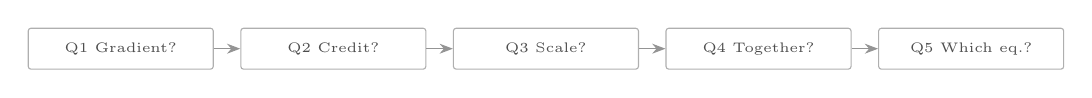
\begin{tikzpicture}
\qnode{0}{q1}{Q1 Gradient?}{1}
\qnode{2.7}{q2}{Q2 Credit?}{2}
\qnode{5.4}{q3}{Q3 Scale?}{3}
\qnode{8.1}{q4}{Q4 Together?}{4}
\qnode{10.8}{q5}{Q5 Which eq.?}{5}
\draw[-{Stealth}, mLightBrown!60] (q1.east) -- (q2.west);
\draw[-{Stealth}, mLightBrown!60] (q2.east) -- (q3.west);
\draw[-{Stealth}, mLightBrown!60] (q3.east) -- (q4.west);
\draw[-{Stealth}, mLightBrown!60] (q4.east) -- (q5.west);
\end{tikzpicture}\end{center}}

%======================================================
\title{Policy-Based Multi-Agent RL}
\subtitle{Learning to Reach the Standoff}
\author{Jinkyoo Park}
\institute{KAIST}
\date{\textit{Lecture 13 --- From coupled Riccati to provable equilibrium learning}}

%======================================================
\begin{document}
%======================================================

\maketitle

%==========================================================
\section{The handoff --- what Lecture 12 left us}
%==========================================================

\begin{frame}{Where we are --- one more axis}
\vspace{2pt}
\begin{center}\footnotesize
\renewcommand{\arraystretch}{1.35}
\begin{tabular}{r|c|c}
 & \textbf{Single Agent} & \textbf{Multi Agent} \\
\hline
\textbf{Static}  & Static optimization & Static Game \\
\hline
\textbf{Dynamic} & Dynamic Optimization \scriptsize(Lec.\ 10) & \cellcolor{mDarkTeal!20}\textbf{Dynamic Game} \scriptsize(Lec.\ 12 $\to$ \alert{13}) \\
\end{tabular}
\end{center}
\smallskip

We stay in the \textbf{bottom-right} cell --- but we move along a \alert{third axis}: from \textbf{model-based} (Lecture 12) to \textbf{data-driven} (today).
\smallskip

\pause
The unfinished business of Lecture 12, stated generally:
\begin{itemize}\setlength\itemsep{2pt}
\item dynamic-game equilibria were \alert{characterized} --- coupled HJB / coupled minimum principles say what a standoff must satisfy;
\item outside special cases, they could not be \alert{computed} --- no general solution procedure exists.
\end{itemize}
\smallskip

\pause
Today asks: can that computation be replaced by \emph{learning from data} --- and what can the learned answer \alert{guarantee}?
\smallskip

{\footnotesize\textcolor{mLightBrown}{Lecture 12's closing line was one instance of this: the building's coupled Riccati as the target of an actor--critic.}}
\end{frame}

\begin{frame}{What we want --- and why we could not have it}
Recall the honest ending of Lecture 12. What we \emph{want} is the \alert{feedback Nash} solution:
\begin{itemize}\setlength\itemsep{1pt}
\item credible from any restart point (\textbf{subgame-perfect}, strongly time-consistent),
\item a \emph{rule} $\gamma^i(t,x)$, not a fragile pre-printed plan.
\end{itemize}
\medskip

\pause
What stood in the way --- three walls:
\begin{itemize}\setlength\itemsep{2pt}
\item \textbf{The model.} Coupled HJB needs $f$ and $g$. Real systems rarely hand them over.
\item \textbf{The closed form.} Outside linear--quadratic, the coupled equations are circular --- no solution formula.
\item \textbf{The dimension.} Even numerically, value fields over $x$ do not survive high dimensions.
\end{itemize}
\medskip

\pause
\begin{center}\large
\alert{The equations exist. The solutions don't.} \quad --- that gap is this lecture.
\end{center}
\end{frame}

\begin{frame}{The translation table --- our coordinate system for today}
Every object of Lecture 12 has a \emph{learned} counterpart. Keep this table in sight --- each paper today fills one of its cells.
\medskip
\begin{center}\scriptsize\renewcommand{\arraystretch}{1.55}
\begin{tabular}{l|l|l}
\textbf{Lecture 12 (model-based)} & \textbf{Lecture 13 (learned)} & \textbf{Who fills it} \\
\hline
coupled value fields $V^i(t,x)$ & centralized critics $Q_i$ & MADDPG, COMA, \dots \\
feedback rules $\gamma^i(t,x)$ & decentralized actors $\pi^i(a_i\,|\,o_i)$ & all of today \\
information structure $\eta^i$ & observation / training design (CTDE) & the whole field \\
equilibrium concept (chosen $\to$ \emph{derived}) & chosen $\to$ \alert{converged to} & HAPPO (NE), HASAC (QRE) \\
\end{tabular}
\end{center}
\medskip

\pause
Read the last row carefully. The \emph{choice} of equilibrium concept remains the modeler's --- exactly as in Lecture 12. What changes is \alert{what the choice buys}: there, coupled conditions to solve by hand; here, an algorithm whose limit points \alert{provably satisfy the chosen concept}.
\smallskip

{\footnotesize\textcolor{mLightBrown}{(The game type --- cooperative, mixed, competitive --- enters through the per-agent rewards, as always.)}}
\end{frame}

\begin{frame}{Two axes, one spectrum --- the scope of today}
Lecture 12 treated information as a binary: open-loop vs.\ feedback. It is really a \alert{spectrum}:
\medskip
\begin{center}
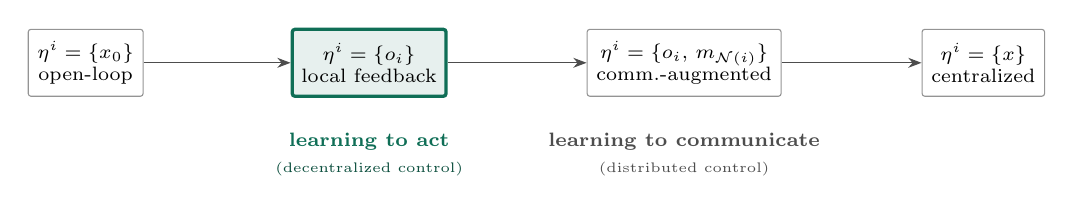
\begin{tikzpicture}[font=\scriptsize, node distance=4pt]
\node[draw=mLightBrown!60, rounded corners=1pt, minimum height=0.85cm, align=center] (a) at (0,0) {$\eta^i=\{x_0\}$\\ open-loop};
\node[draw=mDarkTeal, very thick, fill=mDarkTeal!10, rounded corners=1pt, minimum height=0.85cm, align=center] (b) at (3.6,0) {$\eta^i=\{o_i\}$\\ local feedback};
\node[draw=mLightBrown!60, rounded corners=1pt, minimum height=0.85cm, align=center] (c) at (7.6,0) {$\eta^i=\{o_i,\, m_{\mathcal{N}(i)}\}$\\ comm.-augmented};
\node[draw=mLightBrown!60, rounded corners=1pt, minimum height=0.85cm, align=center] (d) at (11.4,0) {$\eta^i=\{x\}$\\ centralized};
\draw[-{Stealth}, mLightBrown] (a) -- (b); \draw[-{Stealth}, mLightBrown] (b) -- (c); \draw[-{Stealth}, mLightBrown] (c) -- (d);
\node[mDarkTeal, font=\scriptsize\bfseries] at (3.6,-1.0) {learning to act};
\node[mDarkTeal!70!black, font=\tiny] at (3.6,-1.35) {(decentralized control)};
\node[mLightBrown, font=\scriptsize\bfseries] at (7.6,-1.0) {learning to communicate};
\node[mLightBrown, font=\tiny] at (7.6,-1.35) {(distributed control)};
\end{tikzpicture}
\end{center}
\medskip

\pause
\begin{itemize}\setlength\itemsep{2pt}
\item \alert{Learning to act} (today): execution sees only $o_i$. A \emph{reactive pattern} $o_i \to a_i$; all coordination is paid for \textbf{at training time}. This is \textbf{decentralized control}, learned.
\item \alert{Learning to communicate} (closing outlook): agents exchange messages and converge on a joint decision --- a consensus-like inner loop. This is \textbf{distributed control}, learned.
\end{itemize}
\smallskip
{\footnotesize\textcolor{mLightBrown}{Terminology note: these words vary across communities; we use the control-theoretic sense throughout.}}
\end{frame}

\begin{frame}{Recall --- the policy gradient has two faces (Lecture 10)}
For \textbf{one} agent, Lecture 10 gave the gradient of $J(\theta)$ in two equivalent costumes:
\smallskip
\begin{center}\footnotesize\renewcommand{\arraystretch}{1.25}
\begin{tabular}{l|l|l}
 & \textbf{Lagrangian face} (follow trajectories) & \textbf{Eulerian face} (carry a value) \\
\hline
Estimator & REINFORCE: $\nabla\log\pi \cdot \sum_t \gamma^t r_t$ & actor--critic: $\nabla\log\pi\cdot Q_\psi(s,a)$ \\
Object carried & sampled returns along paths & a learned value \emph{field} $Q_\psi$ \\
\end{tabular}
\end{center}
\smallskip

\pause
Today's mainline is \textbf{actor--critic}: the two faces \alert{fused} --- trajectories flowing through a learned field. \alert{Three dials} evolve:
\begin{itemize}\setlength\itemsep{1pt}
\item \textbf{the critic's representation} (the Eulerian object): concat $\to$ attention $\to$ factored; \hfill {\scriptsize Q1--Q3}
\item \textbf{the update's certificate}: none $\to$ monotonic $\to$ convergent; \hfill {\scriptsize Q4}
\item \textbf{the objective's destination}: NE, or QRE$_\alpha$ --- \alert{chosen}, not strengthened. \hfill {\scriptsize Q5}
\end{itemize}
\smallskip
\pause
{\footnotesize\textcolor{mLightBrown}{The Lagrangian face is not gone: its \emph{mathematics} survives in the certificates' proofs (trajectory reweighting, performance-difference --- Act 4); the face itself returns \emph{in person} at the last stop (Act 6).}}
\end{frame}

\begin{frame}{The roadmap --- five questions}
One question per stage. This strip returns at every transition --- watch the highlight move.
\qstrip{0}
\medskip
\begin{itemize}\setlength\itemsep{3pt}
\item \textbf{Q1 --- Can we even compute a gradient?} Independent learners can't. \alert{CTDE} can. \paper{MADDPG, 2017}
\item \textbf{Q2 --- Whose credit is it?} Shared reward hides contributions. \alert{Counterfactual baseline}. \paper{COMA, 2018}
\item \textbf{Q3 --- Can the critic scale?} \alert{Attention} and \alert{factorization}. \paper{MAAC 2019; FACMAC 2021}
\item \textbf{Q4 --- Does improving alone improve together?} \alert{No.} The shock --- and the sequential cure. \paper{MAPPO, HAPPO, MAT, HAML, 2022--24}
\item \textbf{Q5 --- Which equilibrium do we reach?} From NE to \alert{QRE}, by design. \paper{HASAC, 2024}
\end{itemize}
\end{frame}

%==========================================================
\section{What breaks first --- the gradient itself}
%==========================================================

\begin{frame}{The arena --- the stochastic game, recalled}
The data-driven dynamic game is Lecture 7's \textbf{stochastic game}, partially observed:
\begin{itemize}\setlength\itemsep{2pt}
\item shared world: $s_{t+1} \sim P(\,\cdot \mid s_t, a^1_t, \dots, a^N_t)$ --- \emph{everyone's} action moves the same state,
\item per-agent reward $r^i(s_t, a^1_t,\dots,a^N_t)$ and private view $o^i_t = h^i(s_t)$,
\item each agent seeks $\max_{\pi^i} \; \mathbb{E}\big[\sum_t \gamma^t r^i_t\big]$ with a \alert{decentralized} policy.
\end{itemize}
\medskip

\pause
The factorization we commit to (the ``local feedback'' point of the spectrum):
\[
\pi(\mathbf{a}\mid s) \;\approx\; \prod_{i=1}^{N} \pi^i(a_i \mid o_i;\theta_i).
\]
\medskip
\pause
Lecture 12's two breaks are still here --- many goals, limited sight --- but now \alert{$P$, $r$ are unknown}. Only samples.
\end{frame}

\begin{frame}{The naive attempt --- run Lecture 10, $N$ times}
The obvious plan: give every agent its own copy of DDPG / PPO, and let each treat \emph{the rest of the world} --- including the other agents --- as ``the environment.''
\medskip

\begin{center}
\alert{$\text{agent } i:\qquad \max_{\theta_i}\; J_i(\theta_i)\quad \text{pretending } \pi^{-i} \text{ is part of nature.}$}
\end{center}
\medskip

\pause
Notice what this silently assumes. It is Lecture 12's master move --- \emph{``freeze the opponents' rules, then solve a single-agent problem''} --- applied at \textbf{every} learning step.
\medskip

\pause
But in Lecture 12 we froze the opponents \emph{by declaration}, inside a fixed-point argument. Here, \alert{nobody is actually frozen}: all $N$ agents are learning at once.
\medskip

Two things break --- two symptoms of that one assumption: one \alert{temporal} (the world you measured drifts), one \alert{informational} (even in a frozen world, the signal for \emph{joint} success starves).
\end{frame}

\begin{frame}{Failure (i) --- the environment will not sit still}
From agent $i$'s seat, the world it experiences is
\[
P_i\big(s' \mid s, a_i\big) \;=\; \sum_{\mathbf{a}^{-i}} \hl{\pi^{-i}_t(\mathbf{a}^{-i}\mid \cdot)}\; P\big(s' \mid s, a_i, \mathbf{a}^{-i}\big).
\]
The kernel $P_i$ \alert{contains the others' policies} --- and those change every update: the environment is \textbf{non-stationary}, the Markov property is gone.
\medskip

\pause
\textbf{Who gets hurt most: off-policy methods.} A replay buffer stores $(s, a_i, r, s')$ generated under \emph{old} $\pi^{-i}_t$. By the time we replay it, that world no longer exists --- the data quietly lies about the present.
\medskip

\pause
{\footnotesize\textcolor{mLightBrown}{Lecture 7 saw the same disease on the value side: independent Q-learners chase each other's moving targets.}}
\end{frame}

\begin{frame}{Failure (ii) --- the gradient almost never points the right way}
The relevant measure: \alert{how often does a sampled update help?} $\;\langle \hat\nabla J, \nabla J\rangle > 0$ = the step improves $J$.
\smallskip

\textbf{The game} --- a \emph{designed worst case}, the simplest coordination game and policy class:
\begin{center}\small
$a_i \in \{0,1\}$, \quad $P(a_i{=}1) = \theta_i$, \quad $r = \mathbf{1}\{a_1{=}\cdots{=}a_N{=}1\}$, \quad $\theta_i^{\,\mathrm{init}} = 0.5$ \;(uninformed).
\end{center}
\begin{block}{Proposition \hfill {\scriptsize\normalfont\paper{Lowe et al., 2017, Prop.\ 1}}}
\centering
In this game, the single-sample policy gradient satisfies \;\; $\displaystyle P\Big( \big\langle \hat\nabla J,\, \nabla J \big\rangle > 0 \Big) \;\propto\; (0.5)^{N}$.
\end{block}
\smallskip

\pause
\textbf{Why $(0.5)^N$:} the signal flows only through $r$; $r \neq 0$ only when all $N$ \emph{happen} to pick $1$ at once --- probability $(0.5)^N$; every other sample contributes exactly \emph{zero}. $N=10$: $0.1\%$ of updates do anything. \hfill {\footnotesize\textcolor{mLightBrown}{(sketch: Backup 1)}}
\smallskip

\pause
{\footnotesize\textcolor{mLightBrown}{\textbf{Scope:} the \emph{rate} is this construction's; the \emph{mechanism} generalizes: with sparse coordination rewards, informative events are \emph{joint} successes, vanishing multiplicatively in $N$ --- \alert{exponential signal starvation}. And the game is \emph{one-shot}: the disease needs \emph{no} non-stationarity, so it is distinct from Failure (i).}}
\end{frame}

\begin{frame}{The fix, in one line}
Look at the true transition kernel. Policies are nowhere in it:
\[
P\big(s' \mid s, a_1,\dots,a_N,\, \pi_1,\dots,\pi_N\big) \;=\; P\big(s' \mid s, a_1,\dots,a_N\big) \;=\; P\big(s' \mid s, a_1,\dots,a_N,\, \pi_1',\dots,\pi_N'\big).
\]
\medskip
\begin{center}\large
\alert{Condition on \textbf{all actions}, and the environment is stationary again.}
\end{center}
\medskip

\pause
This is \textbf{Centralized Training, Decentralized Execution (CTDE)}:
\begin{itemize}\setlength\itemsep{2pt}
\item \textbf{training:} a critic may see everything --- all observations, all actions ($\Rightarrow$ stationarity restored, \emph{and} every sample informative: the critic maps the \emph{joint}-action landscape, failures included),
\item \textbf{execution:} each actor sees only $o_i$ ($\Rightarrow$ we stay at the spectrum's local-feedback point).
\end{itemize}
\medskip

\pause
It is Lecture 12's ``freeze the opponents' rules'' --- executed not by assumption, but \alert{by conditioning on data}.
\end{frame}

%==========================================================
\section{Stage 1 --- CTDE established (2017--2018)}
%==========================================================

\begin{frame}{MADDPG --- the paradigm paper}
\textbf{Multi-Agent Actor--Critic for Mixed Cooperative--Competitive Environments} \paper{Lowe et al., NeurIPS 2017}
\medskip

Three claims, each mapping onto our coordinate system:
\begin{itemize}\setlength\itemsep{3pt}
\item \textbf{Decentralized execution} --- actors use local observations only: the rules $\gamma^i \to \pi^i(a_i|o_i)$.
\item \textbf{Model-free} --- no $f$, no $g$: the first wall of Lecture 12, removed.
\item \textbf{Cooperative, competitive, or mixed} --- each agent gets its \emph{own} critic $Q_i$, so rewards may conflict: one architecture covers the whole \alert{equilibrium-concept column} of Lecture 12's menu.
\end{itemize}
\medskip
\pause
\begin{center}
\alert{The learned $\{Q_1,\dots,Q_N\}$ are the data-driven coupled value fields $\{V^1,\dots,V^N\}$.}
\end{center}
\end{frame}

\begin{frame}{MADDPG --- the architecture}
\begin{center}
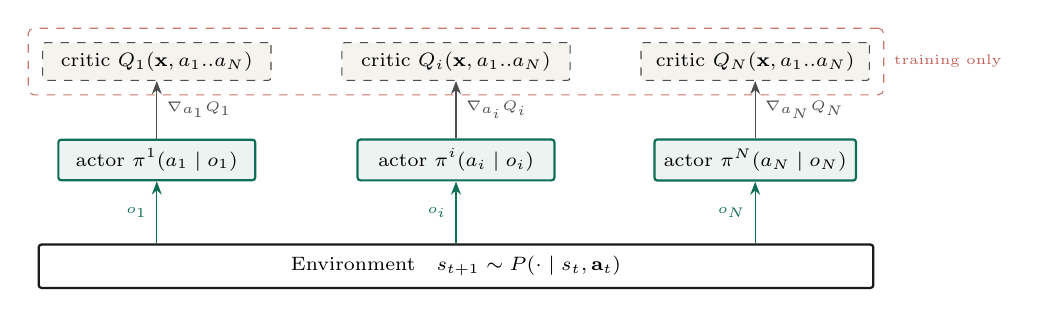
\begin{tikzpicture}[font=\scriptsize, node distance=6pt]
% environment
\node[draw=mDarkBrown, thick, rounded corners=1pt, minimum width=10.6cm, minimum height=0.55cm] (env) at (5.0,0) {Environment \; $s_{t+1}\sim P(\cdot\mid s_t,\mathbf{a}_t)$};
% actors
\node[draw=mDarkTeal, thick, fill=mDarkTeal!8, rounded corners=1pt, minimum width=2.5cm] (a1) at (1.2,1.35) {actor $\pi^1(a_1\mid o_1)$};
\node[draw=mDarkTeal, thick, fill=mDarkTeal!8, rounded corners=1pt, minimum width=2.5cm] (a2) at (5.0,1.35) {actor $\pi^i(a_i\mid o_i)$};
\node[draw=mDarkTeal, thick, fill=mDarkTeal!8, rounded corners=1pt, minimum width=2.5cm] (a3) at (8.8,1.35) {actor $\pi^N(a_N\mid o_N)$};
% critics
\node[draw=mLightBrown, dashed, fill=mPaleBg, rounded corners=1pt, minimum width=2.9cm] (c1) at (1.2,2.6) {critic $Q_1(\mathbf{x},a_1..a_N)$};
\node[draw=mLightBrown, dashed, fill=mPaleBg, rounded corners=1pt, minimum width=2.9cm] (c2) at (5.0,2.6) {critic $Q_i(\mathbf{x},a_1..a_N)$};
\node[draw=mLightBrown, dashed, fill=mPaleBg, rounded corners=1pt, minimum width=2.9cm] (c3) at (8.8,2.6) {critic $Q_N(\mathbf{x},a_1..a_N)$};
\draw[-{Stealth}, mDarkTeal] (env.north -| a1) -- (a1.south) node[midway, left, font=\tiny]{$o_1$};
\draw[-{Stealth}, mDarkTeal] (env.north -| a2) -- (a2.south) node[midway, left, font=\tiny]{$o_i$};
\draw[-{Stealth}, mDarkTeal] (env.north -| a3) -- (a3.south) node[midway, left, font=\tiny]{$o_N$};
\draw[-{Stealth}, mLightBrown] (a1.north) -- (c1.south) node[midway, right, font=\tiny]{$\nabla_{a_1}Q_1$};
\draw[-{Stealth}, mLightBrown] (a2.north) -- (c2.south) node[midway, right, font=\tiny]{$\nabla_{a_i}Q_i$};
\draw[-{Stealth}, mLightBrown] (a3.north) -- (c3.south) node[midway, right, font=\tiny]{$\nabla_{a_N}Q_N$};
% training-only box
\node[draw=mDarkRed!70, dashed, rounded corners=2pt, fit=(c1)(c3), inner sep=5pt, label={[mDarkRed!80, font=\tiny]right:training only}] {};
\end{tikzpicture}
\end{center}
\smallskip

\begin{itemize}\setlength\itemsep{1pt}
\item Solid teal = exists at \textbf{execution}: local observation in, action out. Pure decentralized control.
\item Dashed = exists at \textbf{training} only: each critic sees all observations $\mathbf{x}=(o_1,\dots,o_N)$ and \alert{all actions} --- the conditioning that restores stationarity.
\end{itemize}
\end{frame}

\begin{frame}{MADDPG --- the multi-agent policy gradient}
Lecture 10's deterministic policy gradient, now per player --- written side by side, with the \alert{new arguments} colored \big(as in Lecture 12\big):
\medskip
\begin{columns}[T]
\begin{column}{0.44\linewidth}
\begin{block}{One agent (Lecture 10)}
\centering\small
$\nabla_{\theta} J = \mathbb{E}\Big[ \nabla_{\theta}\mu(s)\; \nabla_{a} Q^{\mu}(s, a)\big|_{a=\mu(s)} \Big]$
\end{block}
\end{column}
\hfill
\begin{column}{0.54\linewidth}
\begin{block}{$N$ players (now)}
\centering
\resizebox{0.97\linewidth}{!}{$\nabla_{\theta_i} J_{\hl i} = \mathbb{E}_{\mathcal{D}}\big[ \nabla_{\theta_i}\mu_i(\hl{o_i})\; \nabla_{a_i} Q_{\hl i}^{\hl{\bm\mu}}\big(\hl{\mathbf{x}}, a_1,\dots,a_N\big)\big|_{a_i=\mu_i(o_i)} \big]$}
\end{block}
\end{column}
\end{columns}
\medskip

\pause
Read the colors:
\begin{itemize}\setlength\itemsep{2pt}
\item the critic is \alert{joint} --- it takes everyone's actions (stationarity), 
\item but the gradient flows only through \alert{agent $i$'s own slot} $a_i$ --- exactly the ``minimize over your own slot'' of Lecture 12's coupled minimum principle, now in gradient form.
\end{itemize}
\smallskip
\pause
{\footnotesize\textcolor{mLightBrown}{Because each $Q_i$ is trained on its own $r_i$, rewards may conflict --- Nash-flavored, not only team.}}
\end{frame}

\begin{frame}{MADDPG --- training the critic}
Each critic regresses on a TD target that uses the \alert{target policies of all agents}:
\[
\mathcal{L}(\theta_i) \;=\; \mathbb{E}_{\mathbf{x},\mathbf{a},r,\mathbf{x}'}\Big[ \big( Q_i^{\bm\mu}(\mathbf{x}, a_1,\dots,a_N) - y_i \big)^2 \Big],
\qquad
y_i \;=\; r_i + \gamma\, Q_i^{\bm\mu'}\big(\mathbf{x}', a_1',\dots,a_N'\big)\Big|_{\hl{a_j' = \mu_j'(o_j)}}.
\]
\medskip

\pause
\textbf{Read the constraint:} forming $y_i$ requires knowing how \emph{every} agent will act next --- i.e.\ access to the others' (target) policies $\mu_j'$.
\begin{itemize}\setlength\itemsep{1pt}
\item fully cooperative training: fine --- policies can simply be shared;
\item competitive settings: you do \alert{not} get your opponent's policy. The assumption must be relaxed $\to$ next slide.
\end{itemize}
\end{frame}

\begin{frame}{MADDPG refinement (a) --- inferring the others' policies}
The TD target $y_i$ needs every opponent's (target) policy; in competition you don't get it --- so \alert{estimate it}. Agent $i$ fits $\hat\mu_{\phi_i^j}$ to agent $j$'s observed behavior by \textbf{entropy-regularized maximum likelihood}:
\[
\mathcal{L}(\phi_i^j) \;=\; -\,\mathbb{E}_{o_j, a_j \sim \mathcal{D}}\big[ \log \hat\mu_{\phi_i^j}(a_j \mid o_j) \big] \;-\; \lambda\, H\big(\hat\mu_{\phi_i^j}\big),
\qquad \text{then } \mu_j' \to \hat\mu_i^{\prime j} \text{ inside } y_i.
\]
\smallskip

\pause
\textbf{Why the entropy term --- two roles of one prior:}
\begin{itemize}\setlength\itemsep{2pt}
\item \textbf{statistical:} finite buffer samples invite overconfident fits; for finite $\mathcal{A}$, $H(p) = \log|\mathcal{A}| - D_{KL}(p \,\|\, \mathrm{unif})$, so the bonus is exactly \alert{smoothing toward uniform} (a MAP / entropic prior);
\item \textbf{structural:} the estimand \emph{drifts} --- agent $j$ keeps learning (Failure (i)'s shadow). A confidently \emph{wrong} $\hat\mu$ makes a confidently wrong bootstrap target; an entropic $\hat\mu$ spreads $y_i$ over plausible opponent actions, \alert{bounding the damage of model error}.
\end{itemize}
\smallskip
{\footnotesize Empirically: despite a visible KL gap to the true policy, success rates match the true-policy oracle.}
\end{frame}

\begin{frame}{MADDPG refinement (b) --- ensembles as a coarse mixed strategy}
\textbf{Problem:} a single deterministic $\mu_i$ is an \alert{exploitable pure strategy}: opponents adapt, and a best response to one frozen opponent collapses against the adapted one. {\footnotesize(Lecture 1: competition may demand \emph{mixed} strategies --- a deterministic policy cannot mix.)}
\smallskip

\pause
\textbf{Construction:} agent $i$ trains \alert{$K$ sub-policies of its own}, $\theta_i^{(1)},\dots,\theta_i^{(K)}$, each with its own buffer $\mathcal{D}_i^{(k)}$; at each \emph{episode start} one is drawn uniformly. The \textbf{objective} is the expected \emph{return} of this mixture --- not a one-shot reward: \; $J_e(\mu_i) = \mathbb{E}_{k \sim \mathrm{unif}(1..K)}\, \mathbb{E}\big[ \textstyle\sum_t \gamma^t r_{i,t} \big]$. The \textbf{estimator} is the centralized critic, \alert{unchanged}, applied per sub-policy:
\[
\nabla_{\theta_i^{(k)}} J_e \;=\; \tfrac{1}{K}\,\mathbb{E}_{\mathbf{x},\mathbf{a}\sim\mathcal{D}_i^{(k)}}\Big[ \nabla_{\theta_i^{(k)}} \mu_i^{(k)}(o_i)\;\, \nabla_{a_i} Q_i^{\bm\mu}\big(\mathbf{x}, a_1,\dots,a_N\big)\big|_{a_i = \mu_i^{(k)}(o_i)} \Big].
\]
{\footnotesize Read carefully: \emph{not} an average over $k$ --- terms $J^{(k')}$, $k'\!\neq\!k$, do not contain $\theta_i^{(k)}$ (one sub-policy per episode), so only the $k$-th survives, with mixture weight $\tfrac1K$. The full gradient is \emph{block-diagonal}: this block is applied for \emph{every} $k$, each on its own $\mathcal{D}_i^{(k)}$.}
\smallskip

\pause
\textbf{Why it works:} episode-level randomization makes the \emph{effective} strategy a mixture --- opponents cannot overfit a \emph{distribution}, and each sub-policy trains against the \alert{population} of behaviors the others' ensembles induce.
\end{frame}

\begin{frame}{What MADDPG leaves open --- two questions}
\textbf{Open question 1 --- shared reward erases credit.} In a \emph{team} game $r_1=\dots=r_N$, all critics learn the \emph{same} function --- every agent is reinforced identically for the team outcome. The lazy agent and the hero get the same pat on the back. \hfill \alert{$\to$ Q2 (COMA)}
\medskip

\pause
\textbf{Open question 2 --- the critic does not scale.} $Q_i(\mathbf{x},a_1..a_N)$ concatenates everything: input grows linearly in $N$, pairwise interactions to be modeled grow \alert{quadratically}, and all agents are weighted \emph{equally, always}. \hfill \alert{$\to$ Q3 (MAAC, FACMAC)}
\medskip

\pause
\qstrip{2}
\end{frame}

\begin{frame}{COMA --- the credit assignment problem}
\textbf{Counterfactual Multi-Agent Policy Gradients} \paper{Foerster et al., AAAI 2018} \quad Fully cooperative: one shared $r(s,\mathbf{u})$.
\smallskip

{\footnotesize\textcolor{mLightBrown}{Notation switch (COMA's): \alert{superscripts now index agents}; $u^i$ = agent $i$'s action ($u$, so letters don't collide), $\tau^i$ = its action--observation history, $\mathbf{u}$ = joint action.}}
\smallskip

\pause
\textbf{The problem, made precise.} The team scores --- one set the screen, one took the shot, one stood still. The joint policy \emph{factorizes}, so its score \emph{decomposes} --- and every term gets the \emph{same} weight:
\[
\pi_\theta(\mathbf{u}\mid\boldsymbol\tau) = \prod_{i=1}^{n}\pi^i(u^i\mid\tau^i)
\;\;\Longrightarrow\;\;
\nabla_{\theta} J = \mathbb{E}\bigg[ \Big( \sum_{i=1}^{n} \nabla_\theta \log \pi^i(u^i\mid\tau^i) \Big)\; \underbrace{\hat A(s,\mathbf{u})}_{\substack{\text{one shared scalar}\\ \text{--- who did what?}}} \bigg]
\]
\pause
$\hat A(s,\mathbf{u})$: \emph{one} team advantage (return $-$ baseline, or $Q-V$) --- \alert{no agent index}; agent $i$'s own share of it drowns in teammate noise as $n$ grows.
\medskip
\pause
\begin{center}
But first, a fair question: \alert{whose $\theta$ is this gradient taken with respect to?}
\end{center}
\end{frame}

\begin{frame}{Reading the gradient --- whose $\theta$?}
Two legitimate readings of $\nabla_\theta J$ --- and the credit problem is the same in both:
\smallskip
\begin{columns}[T]
\begin{column}{0.48\linewidth}
\begin{block}{COMA's case --- shared parameters}
One actor network for all agents (+ agent id): a \emph{single} $\theta$. The sum over $i$ \alert{accumulates onto one vector}: $n$ contributions per step, all weighted by the same $\hat A$.
\end{block}
\end{column}
\hfill
\begin{column}{0.48\linewidth}
\begin{block}{Separate parameters $\theta = (\theta_1,\dots,\theta_n)$}
Cross terms vanish ($\pi^j$ does not contain $\theta_i$), so \emph{block $i$} of the formula is the per-agent gradient:
\centering $\nabla_{\theta_i} J = \mathbb{E}\big[ \nabla_{\theta_i}\log\pi^i(u^i\mid\tau^i)\, \hat A(s,\mathbf{u}) \big]$
\end{block}
\end{column}
\end{columns}
\medskip

\pause
{\footnotesize\textcolor{mLightBrown}{The same block separability as MA-DPG's own-slot gradient, CPG, and the ensembles: one joint objective, per-block gradients --- a pattern worth owning.}}
\smallskip

\pause
\begin{center}
\alert{Either way, the coefficient $\hat A$ is agent-blind: the disease is in the \emph{weight}, not the wiring.}\\[2pt]
So the cure must be a \emph{per-agent} weight: ``how much did \emph{your} action matter, others held fixed?''
\end{center}
\end{frame}

\begin{frame}{Difference rewards --- the idea, and its trap}
\textbf{The classical idea} (difference rewards / aristocrat utility): score agent $i$ by how much the team would have lost had $i$ played its \emph{average} action $\bar u^i$ instead of the one it took:
\[
\text{credit}_i \;\approx\; \underbrace{r(s,\mathbf{u})}_{\text{what happened}} \;-\; \underbrace{r\big(s,(\mathbf{u}^{-i}, \bar u^i)\big)}_{\text{had } i \text{ played its average}}.
\]
\medskip

\pause
\textbf{The trap --- if you make it the \emph{target}.} The ``average self'' $\bar u^i$ is defined \emph{by} $i$'s policy --- the very thing being optimized. Maximizing it chases a goalpost that \alert{moves when you move} --- like beating your own running average, recomputed from your own attempts: a recursive self-consistency loop.
\smallskip

\pause
\textbf{The escape --- put it in the \emph{baseline} slot.} Lecture 10: a baseline may depend on anything \emph{except} $i$'s own sampled action --- it changes \alert{variance, never expectation}. So even as it shifts with the policy, in the baseline slot it cannot \emph{bias} the update, only quiet its noise.
\smallskip
\begin{center}
\alert{Same quantity, different slot: as a \emph{target} it loops; as a \emph{baseline} the trap never closes.}
\end{center}
\end{frame}

\begin{frame}{COMA --- the counterfactual baseline}
\begin{block}{Counterfactual advantage for agent $i$}
\centering
$\displaystyle A^i(s,\boldsymbol\tau,\mathbf{u}) \;=\; Q(s,\boldsymbol\tau,\mathbf{u}) \;-\; \sum_{u'^i} \pi^i\big(u'^i\mid\tau^i\big)\, Q\big(s,\boldsymbol\tau,(\hl{\mathbf{u}^{-i}}, u'^i)\big)$
\end{block}
\medskip

Two moves, named:
\begin{itemize}\setlength\itemsep{2pt}
\item \textbf{freeze the others:} $\hl{\mathbf{u}^{-i}}$ stays at what they actually did;
\item \textbf{marginalize yourself:} average $Q$ over your \emph{own} policy's alternatives $u'^i$.
\end{itemize}
\medskip
\pause
What survives the subtraction is exactly --- and only --- the part of $Q$ that \alert{your action moved}.
\smallskip

{\footnotesize\textcolor{mLightBrown}{Structurally this is a best-response evaluation around the current play --- Lecture 12's reasoning pattern, in expectation form.}}
\end{frame}

\begin{frame}{COMA --- the counterfactual advantage, in one picture}
\centering
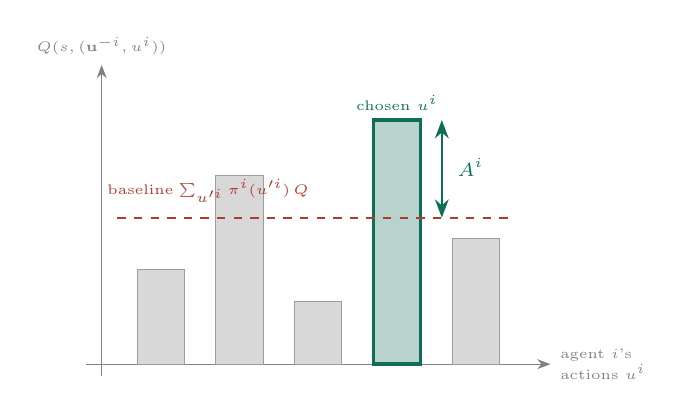
\begin{tikzpicture}[scale=1.0, font=\scriptsize]
\draw[-{Stealth}, mLightBrown!70] (-0.2,0) -- (5.7,0) node[right,font=\tiny, align=left]{agent $i$'s\\ actions $u^i$};
\draw[-{Stealth}, mLightBrown!70] (0,-0.15) -- (0,3.8) node[above,font=\tiny]{$Q(s,(\mathbf{u}^{-i},u^i))$};
\fill[mLightBrown!22, draw=mLightBrown!55] (0.45,0) rectangle (1.05,1.2);
\fill[mLightBrown!22, draw=mLightBrown!55] (1.45,0) rectangle (2.05,2.4);
\fill[mLightBrown!22, draw=mLightBrown!55] (2.45,0) rectangle (3.05,0.8);
\fill[mDarkTeal!30, draw=mDarkTeal, very thick] (3.45,0) rectangle (4.05,3.1);
\fill[mLightBrown!22, draw=mLightBrown!55] (4.45,0) rectangle (5.05,1.6);
\node[font=\tiny, mDarkTeal] at (3.75,3.32) {chosen $u^i$};
\draw[mDarkRed, thick, dashed] (0.2,1.86) -- (5.25,1.86);
\node[mDarkRed, font=\tiny, align=center] at (1.35,2.2) {baseline $\sum_{u'^i}\pi^i(u'^i)\,Q$};
\draw[{Stealth}-{Stealth}, mDarkTeal, thick] (4.32,1.86) -- (4.32,3.1);
\node[mDarkTeal, font=\scriptsize, right] at (4.4,2.5) {$A^i$};
\end{tikzpicture}

\smallskip
{\footnotesize\textcolor{mLightBrown}{Freeze the others, sweep agent $i$'s actions. The dashed line is the \emph{baseline} --- $i$'s policy-averaged value. The counterfactual advantage $A^i$ is the \alert{gap between the action taken and $i$'s own average}: credit for what \emph{this} agent changed, teammates held fixed. \emph{(Redrawn from Foerster et al., 2018.)}}}
\end{frame}

\begin{frame}{Why the baseline is free --- $\mathbb{E}[\,\text{baseline term}\,]=0$}
The baseline $b(s,\mathbf{u}^{-i}) := \sum_{u'^i}\pi^i(u'^i|\tau^i)Q(\cdot)$ does \alert{not depend on $i$'s sampled action $u^i$}. Then:
\medskip

\textbf{Step 1 --- unfold the expectation} (over $i$'s own action):
\[
\mathbb{E}_{u^i\sim\pi^i}\Big[ \nabla_\theta \log\pi^i(u^i\mid\tau^i)\; b(s,\mathbf{u}^{-i}) \Big] = b(s,\mathbf{u}^{-i}) \sum_{u^i} \pi^i(u^i\mid\tau^i)\, \nabla_\theta\log\pi^i(u^i\mid\tau^i).
\]
\pause
\textbf{Step 2 --- likelihood-ratio identity:} $\pi\,\nabla\log\pi = \nabla\pi$, so the sum is $\sum_{u^i}\nabla_\theta\,\pi^i(u^i|\tau^i)$.
\medskip

\pause
\textbf{Step 3 --- normalization:} $\displaystyle \sum_{u^i}\nabla_\theta\,\pi^i = \nabla_\theta \sum_{u^i}\pi^i = \nabla_\theta\, 1 = 0. \qquad\blacksquare$
\medskip

\pause
Bias: zero. Variance: slashed --- teammates' noise is subtracted out. \hfill {\footnotesize\textcolor{mLightBrown}{(full derivation: Backup 2)}}
\end{frame}

\begin{frame}{COMA --- making it computable in one pass}
Naively, the baseline needs $|U|$ extra critic evaluations per agent, per step. COMA reshapes the critic instead:
\medskip
\begin{center}
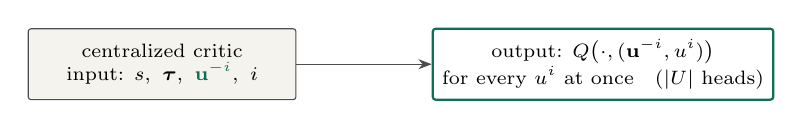
\begin{tikzpicture}[font=\scriptsize]
\node[draw=mLightBrown, fill=mPaleBg, rounded corners=1pt, minimum width=3.4cm, minimum height=0.9cm, align=center] (crit) at (0,0) {centralized critic\\ input: $s,\ \boldsymbol\tau,\ \hl{\mathbf{u}^{-i}},\ i$};
\node[draw=mDarkTeal, thick, rounded corners=1pt, minimum width=3.6cm, minimum height=0.9cm, align=center] (out) at (5.6,0) {output: $Q\big(\cdot,(\mathbf{u}^{-i},u^i)\big)$\\ \alert{for every $u^i$ at once} \; ($|U|$ heads)};
\draw[-{Stealth}, mLightBrown] (crit) -- (out);
\end{tikzpicture}
\end{center}
\medskip

\begin{itemize}\setlength\itemsep{2pt}
\item Others' actions $\mathbf{u}^{-i}$ enter as \emph{inputs}; the output enumerates \emph{my} actions: $|U|$ heads, not $|U|^n$.
\item One forward pass gives both $Q(s,\boldsymbol\tau,\mathbf{u})$ and the entire marginalization sum --- the counterfactual is \alert{exact}, not sampled.
\end{itemize}
\smallskip
\pause
{\footnotesize Actors: one shared GRU network $\pi(u^i\mid\tau^i, \text{agent id})$ --- recurrent, since execution is partially observed.}
\end{frame}

\begin{frame}{Stage 1 closed --- and the next question}
\begin{center}\footnotesize\renewcommand{\arraystretch}{1.5}
\begin{tabular}{l|l|l}
 & \textbf{MADDPG} & \textbf{COMA} \\
\hline
critics & $N$ (one per agent) & $1$ (shared, joint) \\
reward structure & individual $r_i$ (coop / mixed / competitive) & shared $r$ (fully cooperative) \\
actions & continuous (deterministic $\mu_i$) & discrete (stochastic $\pi^i$) \\
credit assignment & --- & counterfactual baseline \\
data regime & off-policy (replay) & on-policy \\
\end{tabular}
\end{center}
\medskip

\pause
\textbf{Stage 1 verdict:} the Eulerian object is now \emph{learned} --- coupled values from data, credit separated. The standoff is being \emph{approximated}.
\medskip

But both critics read the whole world as one flat vector. Can that survive $N=50$?
\smallskip
\qstrip{3}
\end{frame}

%==========================================================
\section{Stage 2 --- the critic learns to scale (2019--2021)}
%==========================================================

\begin{frame}{The scaling problem, concretely}
The Stage-1 critics read a \textbf{flat concatenation} $(o_1,\dots,o_N, a_1,\dots,a_N)$. Three costs:
\begin{itemize}\setlength\itemsep{2pt}
\item input dimension grows in $N$; the pairwise interactions the network must internalize grow \alert{quadratically};
\item every agent's information is processed \alert{equally, all the time};
\item nothing transfers when $N$ changes.
\end{itemize}
\medskip

\pause
\textbf{But dependence is sparse and dynamic.} A football defender does not track all 21 other players --- it tracks \emph{the striker who matters in this phase}, and that changes minute to minute.
\medskip

\pause
\begin{center}
\alert{Wanted: a critic that learns \emph{whom to look at}, and pays only for what it looks at.}
\end{center}
\end{frame}

\begin{frame}{MAAC --- attention enters the critic}
\textbf{Actor-Attention-Critic} \paper{Iqbal \& Sha, ICML 2019}. \; Agent $i$'s critic builds its view of the others in four named steps:
\medskip
\begin{enumerate}\setlength\itemsep{2pt}
\item \textbf{encode:} $e_j = g_j(o_j, a_j)$ for every agent;
\item \textbf{score:} attention weight by query--key similarity \quad $\alpha_j \propto \exp\!\big( e_j^{\top} W_k^{\top} W_q\, e_i \big)$;
\item \textbf{aggregate:} $x_i = \sum_{j\neq i} \alpha_j\, v_j = \sum_{j\neq i} \alpha_j\, h\big(V g_j(o_j,a_j)\big)$;
\item \textbf{output:} $Q_i^{\psi}(\mathbf{o},\mathbf{a}) = f_i\big( g_i(o_i,a_i),\; x_i \big)$.
\end{enumerate}
\medskip

\pause
\begin{itemize}\setlength\itemsep{1pt}
\item $W_q, W_k, V$ are \alert{shared across all agents' critics} (multi-head): value estimation as multi-task regression --- one joint loss trains all $Q_i$ together.
\item \emph{Whom to attend to} is now a \textbf{learned, state-dependent weight}, not an architectural constant.
\end{itemize}
\end{frame}

\begin{frame}{MAAC --- the attention critic, in one picture}
\centering
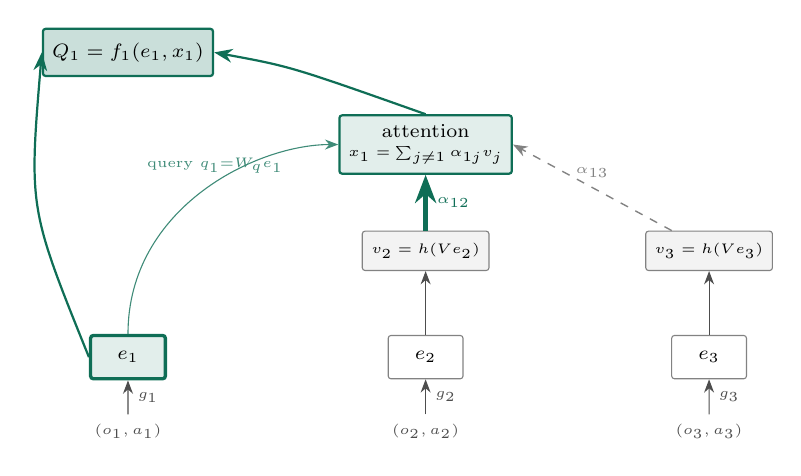
\begin{tikzpicture}[scale=0.9, font=\scriptsize,
  enc/.style={draw=mLightBrown!70, rounded corners=1pt, minimum width=0.95cm, minimum height=0.55cm, align=center},
  self/.style={draw=mDarkTeal, fill=mDarkTeal!12, very thick, rounded corners=1pt, minimum width=0.95cm, minimum height=0.55cm, align=center},
  val/.style={draw=mLightBrown!70, fill=mLightBrown!7, rounded corners=1pt, minimum width=1.55cm, minimum height=0.5cm, align=center, font=\tiny},
  op/.style={draw=mDarkTeal, fill=mDarkTeal!12, thick, rounded corners=1pt, minimum width=2.0cm, minimum height=0.6cm, align=center}]
% inputs
\node[font=\tiny, mLightBrown] (in1) at (-4.0,-1.05) {$(o_1,a_1)$};
\node[font=\tiny, mLightBrown] (in2) at (0.2,-1.05) {$(o_2,a_2)$};
\node[font=\tiny, mLightBrown] (in3) at (4.2,-1.05) {$(o_3,a_3)$};
% encoders
\node[self] (e1) at (-4.0,0.0) {$e_1$};
\node[enc] (e2) at (0.2,0.0) {$e_2$};
\node[enc] (e3) at (4.2,0.0) {$e_3$};
\draw[-{Stealth}, mLightBrown] (in1) -- (e1) node[midway,right,font=\tiny]{$g_1$};
\draw[-{Stealth}, mLightBrown] (in2) -- (e2) node[midway,right,font=\tiny]{$g_2$};
\draw[-{Stealth}, mLightBrown] (in3) -- (e3) node[midway,right,font=\tiny]{$g_3$};
% values (others only)
\node[val] (v2) at (0.2,1.5) {$v_2=h(Ve_2)$};
\node[val] (v3) at (4.2,1.5) {$v_3=h(Ve_3)$};
\draw[-{Stealth}, mLightBrown] (e2) -- (v2);
\draw[-{Stealth}, mLightBrown] (e3) -- (v3);
% attention aggregate
\node[op] (att) at (0.2,3.0) {attention\\[-1pt]{\tiny $x_1=\sum_{j\neq 1}\alpha_{1j}v_j$}};
\draw[-{Stealth}, mDarkTeal, line width=1.6pt] (v2) -- (att) node[midway,right,font=\tiny]{$\alpha_{12}$};
\draw[-{Stealth}, mLightBrown!70, line width=0.5pt, dashed] (v3) -- (att.east) node[midway,above,font=\tiny]{$\alpha_{13}$};
% query from e1
\draw[-{Stealth}, mDarkTeal!80] (e1.north) .. controls (-4.0,2.1) and (-2.2,3.0) .. (att.west) node[pos=0.55,above,font=\tiny]{query $q_1{=}W_q e_1$};
% output
\node[op, fill=mDarkTeal!22] (q1) at (-4.0,4.3) {$Q_1=f_1(e_1,x_1)$};
\draw[-{Stealth}, mDarkTeal, thick] (att.north) .. controls (-1.7,4.1) .. (q1.east);
\draw[-{Stealth}, mDarkTeal, thick] (e1.west) .. controls (-5.4,2.1) .. (q1.west);
\end{tikzpicture}

\smallskip
{\footnotesize\textcolor{mLightBrown}{\textbf{encode} $e_j=g_j(o_j,a_j)$; \textbf{value} $v_j=h(Ve_j)$; \textbf{aggregate} $x_i=\sum_{j\neq i}\alpha_{ij}v_j$ with weights $\alpha_{ij}$ from a query $q_i{=}W_q e_i$; \textbf{output} $Q_i=f_i(e_i,x_i)$. The weights are \emph{learned} --- the critic \alert{chooses whom to look at} ($\alpha_{12}$ thick, $\alpha_{13}$ faint). \emph{(Redrawn from Iqbal \& Sha, 2019.)}}}
\end{frame}

\begin{frame}{MAAC --- the baseline, generalized (one slide vs.\ COMA)}
MAAC also carries a counterfactual baseline --- same spirit, broader reach:
\[
b\big(\mathbf{o}, \mathbf{a}_{\backslash i}\big) = \mathbb{E}_{a_i\sim\pi_i(o_i)}\Big[ Q_i^{\psi}\big(\mathbf{o}, (a_i, \mathbf{a}_{\backslash i})\big) \Big],
\qquad
A_i = Q_i^{\psi}(\mathbf{o},\mathbf{a}) - b(\mathbf{o},\mathbf{a}_{\backslash i}).
\]
\smallskip
\begin{center}\footnotesize\renewcommand{\arraystretch}{1.45}
\begin{tabular}{l|l|l}
 & \textbf{COMA} & \textbf{MAAC} \\
\hline
action spaces & identical across agents & may differ per agent \\
reward & one global $r$ required & per-agent $r_i$ fine \\
others' actions in update & from current rollout (on-policy) & sampled from \alert{current policies} (not buffer) \\
base algorithm & actor--critic & \emph{soft} actor--critic (entropy term) \\
\end{tabular}
\end{center}
\smallskip
\pause
{\footnotesize Sampling teammates from current policies (not the replay buffer) avoids the over-generalization MADDPG can suffer when stale actions poison $Q$.}
\end{frame}

\begin{frame}{MAAC --- does it scale? The evidence}
Cooperative Treasure Collection, growing the team:
\begin{center}\footnotesize\renewcommand{\arraystretch}{1.4}
\begin{tabular}{c|c|c|c}
agents & 4 & 8 & 12 \\
\hline
MAAC improvement over MADDPG+SAC & $+17\%$ & $+98\%$ & \alert{$+208\%$} \\
\end{tabular}
\end{center}
\medskip
The gap \emph{widens} with $N$ --- exactly the signature of linear-vs-quadratic scaling \paper{per-agent input growth: linear with attention, vs.\ quadratic interaction burden with concatenation}.
\medskip

\pause
\textbf{Attention answered ``whom to look at'' --- but the critic is still \emph{one} function} over the joint space: every coordination pattern must be \emph{learned from finite samples}; \alert{none is built in}.
\smallskip
\pause
The other classic way to scale a function: \alert{compositional structure} --- assemble it from per-agent pieces. That idea has a familiar ring: we \emph{paid} for it once before, in Lecture 8.
\end{frame}

\begin{frame}{Recall --- Lecture 8's factorization, and its price}
Value-based MARL assembled the joint value from utilities:
\[
\text{VDN: } Q_{tot} = \textstyle\sum_a Q_a(\tau_a, u_a), \qquad
\text{QMIX: } Q_{tot} = g_\psi\big(s, \{Q_a\}\big), \;\; \frac{\partial Q_{tot}}{\partial Q_a} \ge 0 \;\;(\text{monotone mixing}).
\]
\medskip

\pause
\textbf{Why the monotonicity? The IGM principle.} Execution was \emph{greedy}: each agent plays $\arg\max_{u_a} Q_a$. For that to implement the joint greedy action we needed
\[
\arg\max_{\mathbf{u}} Q_{tot} \;=\; \big( \arg\max_{u_1} Q_1, \dots, \arg\max_{u_N} Q_N \big) \qquad \text{(IGM)},
\]
and monotone mixing is a \emph{sufficient condition} for it --- bought at the price of \alert{restricted representational power}.
\medskip

\pause
\begin{center}
\alert{Keep your eye on that price. Watch how much of it survives the trip to policy land.}
\end{center}
\end{frame}

\begin{frame}{FACMAC --- factor the critic}
\textbf{FACtored Multi-Agent Centralised policy gradients} \paper{Peng et al., NeurIPS 2021}
\smallskip

\textbf{Why factor, when nothing forces you?} No IGM is needed here --- but freedom is not free: a monolithic critic must \emph{learn} all coordination structure from finite samples. FACMAC injects structure \alert{voluntarily}, as an inductive bias --- QMIX's mixing, installed \alert{in the critic}:
\[
Q_{tot}^{\bm\mu}\big(\boldsymbol\tau, \mathbf{u}, s;\, \phi, \psi\big) \;=\; g_\psi\Big( s,\; \big\{ Q_a^{\mu_a}(\tau_a, u_a;\phi_a) \big\}_{a=1}^{n} \Big).
\]
\medskip
\begin{center}
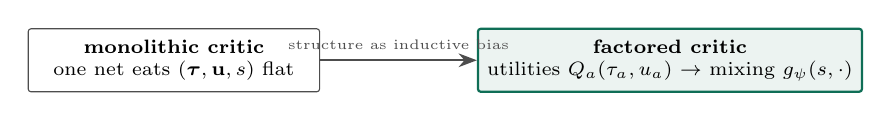
\begin{tikzpicture}[font=\scriptsize]
\node[draw=mLightBrown, rounded corners=1pt, minimum width=3.7cm, minimum height=0.8cm, align=center] (mono) at (0,0) {\textbf{monolithic critic}\\ one net eats $(\boldsymbol\tau,\mathbf{u},s)$ flat};
\node[draw=mDarkTeal, thick, fill=mDarkTeal!8, rounded corners=1pt, minimum width=4.6cm, minimum height=0.8cm, align=center] (fact) at (6.3,0) {\textbf{factored critic}\\ utilities $Q_a(\tau_a,u_a)$ $\to$ mixing $g_\psi(s,\cdot)$};
\draw[-{Stealth}, mLightBrown, thick] (mono) -- (fact) node[midway, above, font=\tiny]{structure as inductive bias};
\end{tikzpicture}
\end{center}
\medskip

\smallskip
{\footnotesize\textcolor{mLightBrown}{One scaling question, two inductive biases: MAAC \emph{learns whom to look at} (dynamic weights); FACMAC \emph{fixes how to assemble} (utilities $+$ mixing). Empirically the factored critic beats the monolithic one --- increasingly so as $n$ grows.}}
\smallskip
\pause
Same equation as Lecture 8 --- but \alert{two statuses changed}: $Q_{tot}$ now supplies \textbf{gradients}, never an \textbf{argmax}; and the structure is \alert{chosen}, not forced. Both changes: next slide.
\end{frame}

\begin{frame}{The hinge --- why the monotonicity constraint dissolves}
Follow the logic in three steps:
\begin{enumerate}\setlength\itemsep{3pt}
\item \textbf{Why Lecture 8 needed monotonicity:} execution = per-agent $\arg\max$ of utilities. IGM is what makes those local argmaxes \emph{reassemble} the joint argmax. Monotone mixing buys IGM.
\item \textbf{What changed:} in actor--critic, \alert{the critic never takes an argmax}. Actions come from the actors; the critic only supplies $\nabla_{\mathbf{u}} Q_{tot}$.
\item \textbf{Therefore:} the factorization is \alert{unconstrained}. Non-monotone mixing is legal --- and FACMAC-nonmonotonic solves tasks that monolithic \emph{and} monotone critics both fail.
\end{enumerate}
\medskip
\pause
\begin{block}{The hinge}
\centering
Lecture 8's constraint was a constraint of \alert{value-based execution}, not of factorization itself.
\end{block}
\smallskip
{\footnotesize\textcolor{mLightBrown}{Honest footnote: \emph{canonical} FACMAC still uses monotone mixing --- as an inductive bias, by choice. Allowed $\neq$ default.}}
\end{frame}

\begin{frame}{FACMAC's second move --- the update dial turns for the first time}
The factored critic settles what $Q_{tot}$ \emph{is}. FACMAC's second contribution asks what actors should \emph{do} with it --- and note the seam: for the first time today, the problem leaves the \alert{representation dial} and touches the \alert{update dial}.
\medskip

\pause
\textbf{The default update has a coordination pathology.} MADDPG-style, each agent climbs its own slot of $Q$ while the others' actions are \alert{pinned from the replay buffer} --- a stale, miscoordinated evaluation point:
\begin{itemize}\setlength\itemsep{2pt}
\item averaged over miscoordinated partners, a ``safe'' suboptimal action outscores the jointly optimal one --- \alert{relative over-generalization};
\item so the team parks where \alert{no single-agent move helps}: a sub-optimal standoff.
\end{itemize}
\smallskip

\pause
{\footnotesize\textcolor{mLightBrown}{MAAC already hinted at the cure --- its baseline samples teammates from \emph{current} policies, not the buffer. CPG takes the hint to its logical end: next slide.}}
\end{frame}

\begin{frame}{FACMAC --- the centralized policy gradient (CPG)}
CPG repairs the \alert{evaluation point}: all actions sampled from \emph{current} policies, one gradient through the whole joint action:
\[
\nabla_{\theta} J(\bm\mu) \;=\; \mathbb{E}_{\mathcal{D}}\Big[ \nabla_{\theta}\,\bm\mu \;\; \nabla_{\bm\mu}\, Q_{tot}^{\bm\mu}\big(\boldsymbol\tau,\, \hl{\mu_1(\tau_1),\dots,\mu_n(\tau_n)},\, s\big) \Big].
\]
Coordinated, simultaneous deviation is possible --- the team can step \emph{together} out of the trap. {\footnotesize(Discrete actions: straight-through Gumbel--Softmax.)}
\smallskip

{\footnotesize\textcolor{mLightBrown}{Joint $\neq$ shared: $\theta = (\theta_1,\dots,\theta_n)$ is a concatenation, $\nabla_\theta\bm\mu$ block-diagonal --- the jointness is the \emph{evaluation point} (everyone's \emph{current} actions, one backward pass through $Q_{tot}$), not parameter sharing.}}
\smallskip

{\footnotesize\textcolor{mLightBrown}{And \emph{not} an on-policy switch: MADDPG and CPG are \emph{both} off-policy (replay). CPG changes the gradient's \alert{evaluation point} (others' \emph{current} vs buffer actions) and factors $Q_{tot}$ --- the data distribution is unchanged.}}
\medskip

\pause
\begin{block}{Hold that thought}
\centering
Simultaneous joint movement is now \emph{possible}. Is it always \emph{safe}? \quad (Act 4 --- the act of the \alert{update dial} --- will say: \alert{no.})
\end{block}
\end{frame}

\begin{frame}{FACMAC --- relative over-generalization, in one picture}
\centering
\begin{columns}[T]
\begin{column}{0.5\linewidth}
\centering
\textbf{\footnotesize the reward landscape}\\[2pt]
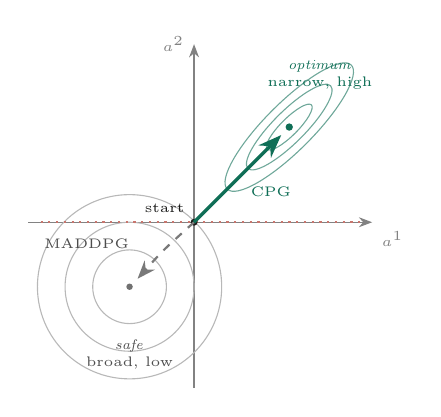
\begin{tikzpicture}[scale=0.78, font=\tiny]
\draw[-{Stealth}, mLightBrown!70] (-2.7,0) -- (2.9,0) node[below right]{$a^1$};
\draw[-{Stealth}, mLightBrown!70] (0,-2.7) -- (0,2.9) node[left]{$a^2$};
% safe broad basin
\foreach \r in {0.6,1.05,1.5}{\draw[mLightBrown!40] (-1.05,-1.05) circle (\r);}
\fill[mLightBrown!80] (-1.05,-1.05) circle (1.5pt);
\node[mLightBrown, align=center] at (-1.05,-2.15) {\emph{safe}\\ broad, low};
% narrow optimum on diagonal ridge
\foreach \r in {0.30,0.56,0.84}{\draw[mDarkTeal!60] (1.55,1.55) ellipse [x radius=\r*1.7, y radius=\r*0.46, rotate=45];}
\fill[mDarkTeal] (1.55,1.55) circle (1.7pt);
\node[mDarkTeal, align=center] at (2.05,2.4) {\emph{optimum}\\ narrow, high};
% agent 1's slice (a2 fixed at start)
\draw[mDarkRed!70, dotted, thick] (-2.5,0) -- (2.7,0);
% start + moves
\fill[mDarkBrown] (0,0) circle (1.6pt) node[above left]{start};
\draw[-{Stealth}, mLightBrown!75, dashed, thick] (0,0) .. controls (-0.5,-0.45) .. (-0.92,-0.92);
\node[mLightBrown] at (-1.75,-0.35) {MADDPG};
\draw[-{Stealth}, mDarkTeal, very thick] (0,0) .. controls (0.7,0.7) .. (1.42,1.42);
\node[mDarkTeal] at (1.25,0.5) {CPG};
\end{tikzpicture}
\end{column}
\begin{column}{0.5\linewidth}
\centering
\textbf{\footnotesize what agent 1 sees on the slice}\\[2pt]
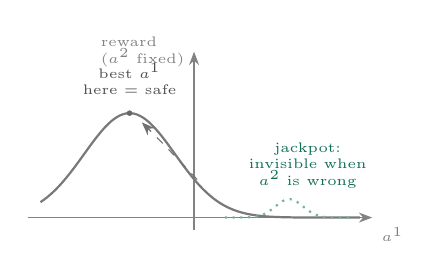
\begin{tikzpicture}[scale=0.78, font=\tiny]
\draw[-{Stealth}, mLightBrown!70] (-2.7,0) -- (2.9,0) node[below right]{$a^1$};
\draw[-{Stealth}, mLightBrown!70] (0,-0.2) -- (0,2.7) node[left, align=left]{reward\\ ($a^2$ fixed)};
\draw[mLightBrown!75, thick, domain=-2.5:2.7, smooth, samples=90] plot (\x, {1.7*exp(-((\x+1.05)*(\x+1.05))/1.1)});
\draw[mDarkTeal!55, thick, dotted, domain=0.5:2.6, smooth, samples=70] plot (\x, {0.30*exp(-((\x-1.55)*(\x-1.55))/0.10)});
\fill[mLightBrown!85] (-1.05,1.7) circle (1.3pt);
\node[mLightBrown, align=center] at (-1.05,2.25) {best $a^1$\\ here = safe};
\node[mDarkTeal, align=center] at (1.85,0.85) {jackpot:\\ invisible when\\ $a^2$ is wrong};
\draw[-{Stealth}, mLightBrown!80, dashed] (0.05,0.62) .. controls (-0.5,1.2) .. (-0.85,1.55);
\end{tikzpicture}
\end{column}
\end{columns}
\smallskip
{\footnotesize\textcolor{mLightBrown}{Two hills: a broad \emph{safe} region (low) and a narrow diagonal \emph{optimum} (high) that needs both agents aligned. \textbf{Why MADDPG drifts:} with the partner's $a^2$ fixed at a wrong value, agent 1's own slice (right) shows only the broad safe hump --- the jackpot is \alert{invisible until both move}. So per-agent steps slide to safe; the \emph{joint} CPG step climbs the ridge. \emph{(Schematic, in the spirit of Peng et al., 2021.)}}}
\end{frame}

\begin{frame}{Aside --- MAMuJoCo: one robot as many agents}
FACMAC's benchmark contribution: take a single MuJoCo robot, read its \textbf{body graph}, and assign \alert{each joint group to an agent} --- continuous, fully cooperative control where coordination is physical.
\medskip

\begin{itemize}\setlength\itemsep{2pt}
\item One plant, many actuators, one shared objective --- exactly Lecture 12's \emph{building with three controllers}, now as a learning benchmark.
\item The idea ``a robot \emph{is} a multi-agent system'' has an older life in graph-structured policies (NerveNet and kin); here it is industrialized into the standard continuous-MARL testbed.
\end{itemize}
\medskip
\pause
{\footnotesize\textcolor{mLightBrown}{Why we will see it again: MAMuJoCo agents are \emph{heterogeneous} (different joints, different action spaces) --- the setting where parameter sharing fails and Stage 3's theory will earn its keep.}}
\end{frame}

\begin{frame}{Stage 2 closed --- and the unease}
\textbf{What we now have:} critics that scale --- attention chooses \emph{whom to read}, factorization chooses \emph{how to assemble}; actors that move jointly (CPG).
\medskip

\pause
\textbf{What we do not have:} a single \alert{guarantee}. Nothing so far promises that a policy update --- any of them --- makes the team better.
\medskip

\begin{center}\large
If every agent improves its own policy, does the team improve?
\end{center}
\medskip
\pause
The next stage begins with the empirical high-water mark of ``just do the simple thing'' --- and then shows precisely where the simple thing has no floor under it.
\smallskip
\qstrip{4}
\end{frame}

%==========================================================
\section{The second shock --- and the theory that answers it (2022--2024)}
%==========================================================

\begin{frame}{Stage 3 --- the act of the update dial}
\qstrip{4}
\medskip

The previous slide asked: \emph{if every agent improves its own policy, does the team improve?} This whole act is the answer --- in three beats.

\medskip
\pause
\textbf{1. The promise} \,(one agent): PPO/TRPO guarantee \alert{monotonic improvement} --- inside a trust region, an update is \emph{never worse}.

\smallskip
\pause
\textbf{2. The shock} \,(many agents, at once): let everyone take their improving step \emph{simultaneously}, and the \emph{joint} return can \alert{drop} --- each agent's promise assumed the others stood still.

\smallskip
\pause
\textbf{3. The cure} \,(take turns): update \emph{sequentially}, each agent accounting for those before it --- the individual gains \alert{telescope} into a guaranteed team improvement, and the fixed point is a \alert{Nash equilibrium}.

\medskip
\pause
{\footnotesize\textcolor{mLightBrown}{Roadmap: \textbf{MAPPO} (simple thing works) $\to$ \textbf{the shock} (no floor) $\to$ \textbf{sequential cure} (HATRPO / HAPPO: monotonic $+$ Nash) $\to$ one \textbf{framework} (HAML), one \textbf{sequence model} (MAT).}}
\end{frame}

\begin{frame}{MAPPO and IPPO --- the simplest lift of PPO}
\textbf{Setup.} $n$ cooperative agents; agent $i$ acts only on its local observation $o_i$.
\medskip

\pause
\textbf{The idea: run single-agent PPO, once per agent.} Each agent carries a policy $\pi_\theta(a_i\mid o_i)$ trained with the ordinary clipped-PPO objective; for \emph{homogeneous} agents the weights $\theta$ are \alert{shared} (one network $+$ agent id). \emph{No new algorithm} --- PPO, copied across agents.
\medskip

\pause
\textbf{Two variants, differing only in what the \emph{critic} sees:}
\begin{itemize}\setlength\itemsep{3pt}
\item \textbf{IPPO} --- \emph{independent}: a local value $V_\phi(o_i)$; each agent learns on its own.
\item \textbf{MAPPO} --- \emph{centralized}: a global value $V_\phi(s)$; the critic sees the whole state (CTDE).
\end{itemize}
\medskip

\pause
\begin{center}
\alert{The policies are plain PPO --- the only design choice is the critic's input.}
\end{center}
\end{frame}

\begin{frame}{MAPPO --- the surprising effectiveness of doing less}
\textbf{The Surprising Effectiveness of PPO in Cooperative Multi-Agent Games} \paper{Yu et al., NeurIPS 2022}
\medskip

We have the algorithm; now \emph{why it matters}. The paper's claim is purely empirical ---
\begin{itemize}\setlength\itemsep{2pt}
\item well-tuned PPO with a centralized value function matches or beats strong off-policy methods (MPE, SMAC, GRF, Hanabi)

\item with \emph{comparable sample budgets}, no exotic architecture, minimal tuning.
\end{itemize}
\medskip

\pause
Its cultural role: after years of increasingly intricate machinery, the field's strongest cooperative baseline turned out to be \emph{the simplest thing, done carefully}.
\medskip

\pause
Which sharpens the real question: if the simple thing works this well\,---\,\alert{what exactly was the machinery for?} Hold on; first, where does MAPPO hide its centralization?
\end{frame}

\begin{frame}{MAPPO vs.\ IPPO --- where the centralization hides}
Both train \textbf{local} policies $\pi_\theta(a_i\mid o_i)$ with the clipped objective; both share parameters across (homogeneous) agents. The \emph{only} difference is the \alert{value function's input}:
\[
\text{IPPO: } V_\phi(o_i) \qquad\text{vs.}\qquad \text{MAPPO: } V_\phi(\hl{s}) \;\;\text{(global / agent-specific global state)}.
\]
\medskip

\pause
Why this is legal CTDE: $V_\phi$ is used \textbf{only to build advantages during training} --- it never acts. So it may see everything, and execution stays decentralized.
\medskip

\[
L(\theta) = \tfrac{1}{Bn}\textstyle\sum_{i,k} \min\!\Big( r^{(k)}_{\theta,i} A^{(k)}_i,\; \mathrm{clip}\big(r^{(k)}_{\theta,i}, 1\pm\epsilon\big) A^{(k)}_i \Big) + \sigma\,S[\pi_\theta], 
\qquad r^{(k)}_{\theta,i} = \frac{\pi_\theta(a^{(k)}_i\mid o^{(k)}_i)}{\pi_{\theta_{old}}(a^{(k)}_i\mid o^{(k)}_i)}.
\]
{\footnotesize plus a clipped value loss on $V_\phi$ with targets $\hat R$ (GAE).}
\end{frame}

\begin{frame}{MAPPO --- the five factors that actually matter}
The paper's lasting practical contribution --- five implementation levers:
\begin{enumerate}\setlength\itemsep{2pt}
\item \textbf{value normalization} (running statistics on targets);
\item \textbf{value input}: agent-specific global state (concat local + global, pruned of redundancy);
\item \textbf{training-data usage}: hard tasks $\Rightarrow$ fewer epochs, avoid mini-batch splitting;
\item \textbf{clipping} $\epsilon$ small ($< 0.2$): keep updates conservative;
\item \textbf{batch size}: large first, then trade for sample efficiency.
\end{enumerate}
\medskip
\pause
{\footnotesize\textcolor{mLightBrown}{Read levers 3--5 together: they all say \emph{keep the simultaneous steps small}. The practitioners had felt the disease before the theorists named it. Next slide names it.}}
\end{frame}

\begin{frame}{It works. But what is promised?}
Picture one MAPPO iteration: \alert{all $n$ agents update simultaneously}, each maximizing its own clipped surrogate, each surrogate computed \textbf{against teammates frozen at $\theta_{old}$}.
\medskip

\pause
Each agent ends its step holding a certificate: \emph{``relative to the world I measured, I improved.''}
\medskip

\pause
But the world each one measured \textbf{no longer exists} --- everyone else moved too.
\medskip

\begin{itemize}\setlength\itemsep{2pt}
\item TRPO's monotonic-improvement bound is a \alert{single-agent theorem}: it bounds the damage of \emph{your own} policy shift, not of $n-1$ simultaneous shifts in the joint distribution.
\item Question: can $n$ individually-certified improvements combine into a joint \emph{deterioration}?
\end{itemize}
\medskip
\pause
\begin{center}\large \alert{Yes. By hand, on one line of algebra --- next slide.}\end{center}
\end{frame}

\begin{frame}{The shock --- improving alone, worsening together}
\begin{columns}[c]
\begin{column}{0.52\linewidth}
\small
Two agents, one joint reward to \textbf{maximize}: $r(a^1,a^2) = a^1 a^2$. Current point $(1,-1)$, so $r=-1$. Gradients: $\partial_{a^1} r = a^2 = -1$, \; $\partial_{a^2} r = a^1 = 1$. Each agent takes its ascent step with size $\eta = 3$:
\medskip

\textbf{Agent 1 alone:} $a^1 \to -2$:\; $r = (-2)(-1) = \hl{2}$ \;\checkmark
\smallskip

\textbf{Agent 2 alone:} $a^2 \to 2$:\; $r = (1)(2) = \hl{2}$ \;\checkmark
\smallskip

\textbf{Both together:} $(-2, 2)$:\; $r = \alert{-4}$ \;\texttimes
\medskip

\pause
Both certificates were \emph{true}. Both premises --- ``the other stays put'' --- were \emph{false}.
\end{column}
\begin{column}{0.46\linewidth}
\centering
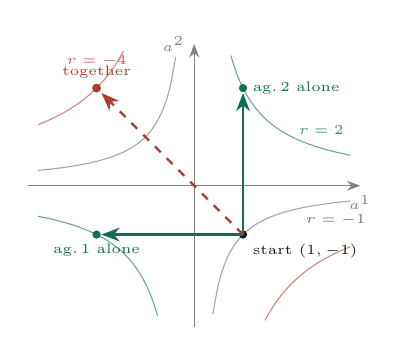
\begin{tikzpicture}[scale=0.62, font=\tiny]
\draw[-{Stealth}, mLightBrown!70] (-3.4,0) -- (3.4,0) node[below]{$a^1$};
\draw[-{Stealth}, mLightBrown!70] (0,-2.9) -- (0,2.9) node[left]{$a^2$};
% contours r = -1 : y=-1/x
\draw[mLightBrown!50, domain=0.38:3.2, smooth] plot (\x, {-1/\x});
\draw[mLightBrown!50, domain=-3.2:-0.38, smooth] plot (\x, {-1/\x});
% r = 2 : y=2/x
\draw[mDarkTeal!60, domain=0.75:3.2, smooth] plot (\x, {2/\x});
\draw[mDarkTeal!60, domain=-3.2:-0.75, smooth] plot (\x, {2/\x});
% r = -4 : y=-4/x
\draw[mDarkRed!60, domain=1.45:3.2, smooth] plot (\x, {-4/\x});
\draw[mDarkRed!60, domain=-3.2:-1.45, smooth] plot (\x, {-4/\x});
\node[mLightBrown!80] at (2.9,-0.7) {$r=-1$};
\node[mDarkTeal!80] at (2.6,1.15) {$r=2$};
\node[mDarkRed!80] at (-2.0,2.55) {$r=-4$};
% points
\fill[mDarkBrown] (1,-1) circle (2.4pt) node[below right]{start $(1,-1)$};
\fill[mDarkTeal] (-2,-1) circle (2.4pt) node[below]{ag.\,1 alone};
\fill[mDarkTeal] (1,2) circle (2.4pt) node[right]{ag.\,2 alone};
\fill[mDarkRed] (-2,2) circle (2.6pt) node[above]{together};
\draw[-{Stealth}, mDarkTeal, thick] (1,-1) -- (-1.9,-1);
\draw[-{Stealth}, mDarkTeal, thick] (1,-1) -- (1,1.9);
\draw[-{Stealth}, mDarkRed, thick, dashed] (1,-1) -- (-1.9,1.9);
\end{tikzpicture}
\end{column}
\end{columns}
\smallskip
{\footnotesize\textcolor{mLightBrown}{Construction in the spirit of Kuba et al.\ (2022), Fig.\ 1. With infinitesimal steps this bilinear game does \emph{not} fail --- the disease lives at \textbf{finite} step sizes, exactly where surrogate-justified methods (TRPO/PPO) operate.}}
\end{frame}

\begin{frame}{The disease, third costume}
\begin{center}
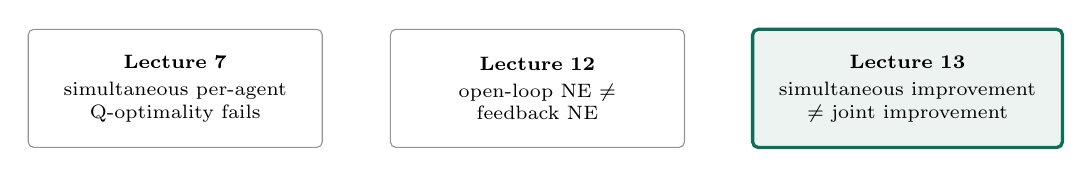
\begin{tikzpicture}[font=\scriptsize, node distance=10pt]
\node[draw=mLightBrown!60, rounded corners=2pt, align=center, minimum height=1.5cm, text width=3.5cm] (a) at (0,0) {\textbf{Lecture 7}\\[2pt] simultaneous per-agent\\ Q-optimality fails};
\node[draw=mLightBrown!60, rounded corners=2pt, align=center, minimum height=1.5cm, text width=3.5cm] (b) at (4.6,0) {\textbf{Lecture 12}\\[2pt] open-loop NE $\neq$\\ feedback NE};
\node[draw=mDarkTeal, very thick, fill=mDarkTeal!8, rounded corners=2pt, align=center, minimum height=1.5cm, text width=3.7cm] (c) at (9.3,0) {\textbf{Lecture 13}\\[2pt] simultaneous improvement\\ $\neq$ joint improvement};
\end{tikzpicture}
\end{center}
\medskip

One disease, three costumes:
\begin{center}\large
\alert{Optimality computed while the others move is voided the moment they do.}
\end{center}
\medskip
\pause
And as in Lectures 7 and 12, the cure will not be a patch --- it will be a \textbf{restructuring of what we ask for}: not ``everyone improves at once,'' but something order-aware. \alert{From here, every remaining slide builds that cure.}
\end{frame}

\begin{frame}{The answer to the shock --- one paper, one identity}
The diagnosis is settled: \alert{simultaneous improvement carries no team guarantee}.
\medskip

\pause
The fix arrived in a single paper:
\begin{center}
\textbf{Trust Region Policy Optimisation in Multi-Agent Reinforcement Learning}\\[2pt]
\paper{Kuba et al., ICLR 2022}
\end{center}
whose aim is exactly to \alert{recover the single-agent monotonic-improvement guarantee for the whole team}.
\medskip

\pause
Its algorithms \textbf{HATRPO / HAPPO} --- and a clear-eyed look at where parameter sharing fits (next slide) --- rest on \emph{one theoretical identity}. The following slides build that identity, the \textbf{Multi-Agent Advantage Decomposition Lemma}, and then cash it.
\end{frame}

\begin{frame}{Parameter sharing answers a different question}
\textbf{Give sharing its due.} For \emph{homogeneous} agents, one shared policy $\pi_\theta(a_i\mid o_i)$ is often \alert{optimal} --- and the standard choice. Agents see different \emph{observations} (plus an index), so the \emph{same} network outputs different actions: roles and cooperation emerge with \emph{no} per-agent parameters. (Ten identical AMRs: share one policy.)
\medskip

\pause
\textbf{But that is about \emph{representation}; the shock was about the \emph{guarantee}.} Sharing never certifies that a team update improves the team --- and with \emph{one} $\theta$ you \alert{cannot move one agent while holding the rest fixed} (they are the same parameters). The simultaneous movement that caused the shock is \emph{baked in}.
\medskip

\pause
\begin{center}
\alert{The guarantee comes from \emph{how} we update, not how we parameterize.}
\end{center}
To improve agents \emph{one at a time} --- so the gains telescope --- we need separately-adjustable policies. That update rule needs one new piece of mathematics.
\smallskip
{\footnotesize\textcolor{mLightBrown}{(The shared class is limiting only when agents cannot tell themselves apart --- identical observations, no index --- where the best shared policy can hit $2/2^n$ \paper{Kuba et al., 2022, Prop.\ 1}. With distinct observations, a non-issue.)}}
\end{frame}

\begin{frame}{Reading the notation --- an ordering, and who has committed}
The promised \emph{new mathematics} needs vocabulary. Fix an \alert{ordering} of the agents $i_1,i_2,\dots,i_n$ (a turn order); we score them \emph{as if they commit their actions one at a time, down this order}.
\medskip

\begin{center}
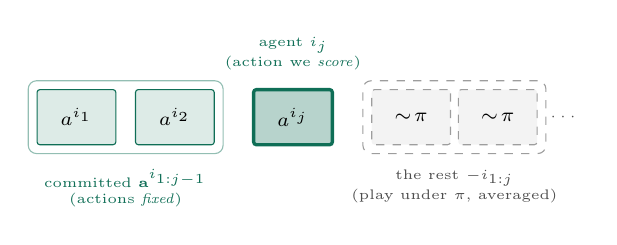
\begin{tikzpicture}[font=\scriptsize,
  comm/.style={draw=mDarkTeal, fill=mDarkTeal!14, rounded corners=1pt, minimum width=1.0cm, minimum height=0.7cm},
  cur/.style={draw=mDarkTeal, very thick, fill=mDarkTeal!30, rounded corners=1pt, minimum width=1.0cm, minimum height=0.7cm},
  rest/.style={draw=mLightBrown!55, dashed, fill=mLightBrown!7, rounded corners=1pt, minimum width=1.0cm, minimum height=0.7cm}]
\node[comm] (b1) at (0,0) {$a^{i_1}$};
\node[comm] (b2) at (1.25,0) {$a^{i_2}$};
\node[cur]  (b3) at (2.75,0) {$a^{i_j}$};
\node[rest] (b4) at (4.25,0) {$\sim\!\pi$};
\node[rest] (b5) at (5.35,0) {$\sim\!\pi$};
\node[font=\tiny, mLightBrown] at (6.2,0) {$\cdots$};
\node[draw=mDarkTeal!45, rounded corners=3pt, fit=(b1)(b2), inner sep=3pt] (gc) {};
\node[font=\tiny, mDarkTeal, below=2pt of gc, align=center] {committed $\mathbf{a}^{i_{1:j-1}}$\\(actions \emph{fixed})};
\node[font=\tiny, mDarkTeal, align=center, above=3pt of b3] {agent $i_j$\\(action we \emph{score})};
\node[draw=mLightBrown!55, dashed, rounded corners=3pt, fit=(b4)(b5), inner sep=3pt] (gr) {};
\node[font=\tiny, mLightBrown, below=2pt of gr, align=center] {the rest $-i_{1:j}$\\(play under $\pi$, averaged)};
\end{tikzpicture}
\end{center}
\medskip

{\footnotesize
\begin{itemize}\setlength\itemsep{2pt}
\item $i_j$ = the agent in \emph{position} $j$;\quad $i_{1:m}=(i_1,\dots,i_m)$ = the first $m$ of the order.
\item \textbf{Superscript} on $\mathbf{a}$ or $Q$ = \emph{who has committed} (action fixed): $\;\mathbf{a}^{i_{1:m}}=(a^{i_1},\dots,a^{i_m})$.
\item The complement $-i_{1:m}$ = everyone else; they \emph{still play under $\pi$} and are averaged out. Subscript $\pi$ = under the joint policy.
\end{itemize}}
\end{frame}

\begin{frame}{Recall and define --- advantages, alone and in groups}
\textbf{Recall (Lecture 10):} $A_\pi(s,\mathbf{a}) = Q_\pi(s,\mathbf{a}) - V_\pi(s)$ --- ``how much better than average is this action?'' (estimated by GAE).
\medskip

\pause
\textbf{Define (new):} for an ordered subset $i_{1:m}$ of agents,
\begin{itemize}\setlength\itemsep{4pt}
\item \emph{multi-agent value of a partial action:} \; $\displaystyle Q^{i_{1:m}}_{\pi}\big(s, \mathbf{a}^{i_{1:m}}\big) \;=\; \mathbb{E}_{\mathbf{a}^{-i_{1:m}} \sim \pi^{-i_{1:m}}}\big[ Q_\pi(s, \mathbf{a}) \big]$ \hfill {\footnotesize(the rest play on)}
\item \emph{multi-agent advantage:} \; $A^{i_{1:m}}_{\pi}\big(s,\mathbf{a}^{i_{1:m}}\big) = Q^{i_{1:m}}_{\pi}(s,\mathbf{a}^{i_{1:m}}) - V_\pi(s)$
\item \emph{conditional local advantage of agent $i_j$, given its predecessors:}
\[
A^{i_j}_{\pi}\big(s,\, \mathbf{a}^{i_{1:j-1}},\, a^{i_j}\big) \;=\; Q^{i_{1:j}}_{\pi}\big(s, \mathbf{a}^{i_{1:j}}\big) \;-\; Q^{i_{1:j-1}}_{\pi}\big(s, \mathbf{a}^{i_{1:j-1}}\big).
\]
\end{itemize}
\medskip
\pause
Read the last line in words: \alert{the marginal contribution of $i_j$'s action, on top of what the predecessors already committed.} (Convention: $Q^{i_{1:0}}_\pi := V_\pi(s)$.)
\end{frame}

\begin{frame}{The Multi-Agent Advantage Decomposition Lemma}
\begin{block}{Lemma \hfill {\scriptsize\normalfont\paper{Kuba et al., ICLR 2022, Lemma 1}}}
\centering
For \emph{any} cooperative Markov game, \emph{any} state $s$, \emph{any} ordering $i_{1:n}$, and \emph{any} joint action:
\[
A^{i_{1:n}}_{\pi}\big(s, \mathbf{a}^{i_{1:n}}\big) \;=\; \sum_{j=1}^{n} A^{i_j}_{\pi}\big(s,\, \mathbf{a}^{i_{1:j-1}},\, a^{i_j}\big).
\]
\end{block}
\medskip

\textbf{In words:} the joint contribution equals the sum of \emph{sequential marginal} contributions --- an accounting identity (decompose a team's surplus by adding members one at a time).
\smallskip

\pause
\textbf{Why it is the engine of the cure:} it converts the hard goal ``raise the \emph{joint} return'' into ``raise each \emph{ordered marginal} term.'' Improve the summands \emph{in order} and the joint advantage is positive --- exactly what the sequential update will exploit (next slides).
\smallskip

\pause
\alert{And it needs no assumptions} --- no IGM, no monotonicity. {\footnotesize\textcolor{mLightBrown}{(Lecture 8 paid for value decomposition with structure; this identity is free --- full comparison after the proof.)}}
\end{frame}

\begin{frame}{Proof --- a telescope}
\textbf{Step 1 --- definition unfolding.} Each summand is, by the definition on the previous slide, a difference of partial-action values:
\[
A^{i_j}_{\pi}\big(s, \mathbf{a}^{i_{1:j-1}}, a^{i_j}\big) \;=\; Q^{i_{1:j}}_{\pi}\big(s,\mathbf{a}^{i_{1:j}}\big) - Q^{i_{1:j-1}}_{\pi}\big(s,\mathbf{a}^{i_{1:j-1}}\big).
\]
\pause
\textbf{Step 2 --- telescoping sum.} Adjacent terms cancel in pairs:
\[
\sum_{j=1}^{n} \Big[ Q^{i_{1:j}}_{\pi} - Q^{i_{1:j-1}}_{\pi} \Big]
= \cancel{Q^{i_{1:1}}} - Q^{i_{1:0}} + \cancel{Q^{i_{1:2}}} - \cancel{Q^{i_{1:1}}} + \dots + Q^{i_{1:n}} - \cancel{Q^{i_{1:n-1}}}
= Q^{i_{1:n}}_{\pi} - Q^{i_{1:0}}_{\pi}.
\]
\pause
\textbf{Step 3 --- read off the ends.} $Q^{i_{1:n}}_{\pi}(s,\mathbf{a}) = Q_\pi(s,\mathbf{a})$ (everyone specified) and $Q^{i_{1:0}}_{\pi} = V_\pi(s)$ (no one specified), so the sum is $Q_\pi - V_\pi = A^{i_{1:n}}_{\pi}(s,\mathbf{a})$. \hfill $\blacksquare$

\medskip
\pause
{\footnotesize Three named moves --- definition unfolding, telescoping, boundary reading. Nothing else. \textcolor{mLightBrown}{(fully expanded: Backup 3)}}
\end{frame}

\begin{frame}{IGM vs.\ Advantage Decomposition --- the price changed currency}
\begin{center}\footnotesize\renewcommand{\arraystretch}{1.55}
\begin{tabular}{l|l|l}
 & \textbf{IGM (Lecture 8)} & \textbf{Adv.\ Decomposition (today)} \\
\hline
what is decomposed & joint \emph{value} $Q_{tot}$ & joint \emph{advantage} $A^{i_{1:n}}$ \\
holds because of & an \alert{assumption} (architectural) & an \alert{identity} (always true) \\
why it was needed & greedy decentralized execution ($\arg\max$) & sequential conditioning \\
the price paid & restricted representation (monotone mixing) & an \alert{ordering} (sequential updates) \\
who pays & the network, forever & the algorithm, once per iteration \\
\end{tabular}
\end{center}
\medskip

\pause
\begin{block}{The structural insight of this lecture}
\centering
The cost of decomposition did not vanish ---\\ it \alert{changed currency}: from \textbf{structure} to \textbf{order}.
\end{block}
\medskip
\pause
And ``order'' is a currency an algorithm can actually afford. Next: spend it.
\end{frame}

\begin{frame}{From lemma to algorithm --- the sequential sweep}
\textbf{Corollary of the lemma.} Fix an order. Let each agent, \emph{in turn}, choose an update that makes its \alert{conditional} local advantage positive --- conditioned on the predecessors' \emph{already-updated} behavior. Then every summand is positive, so the \textbf{joint} advantage is positive.
\medskip

\begin{center}
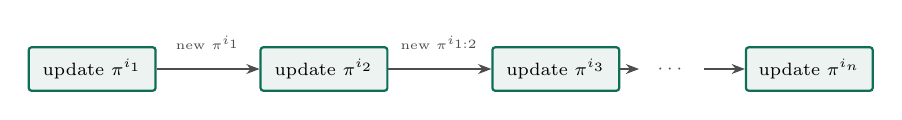
\begin{tikzpicture}[font=\scriptsize, scale=0.92, transform shape,
  ub/.style={draw=mDarkTeal, thick, fill=mDarkTeal!8, rounded corners=1pt, minimum width=1.75cm, minimum height=0.6cm}]
\node[ub] (u1) at (0,0) {update $\pi^{i_1}$};
\node[ub] (u2) at (3.2,0) {update $\pi^{i_2}$};
\node[ub] (u3) at (6.4,0) {update $\pi^{i_3}$};
\node[mLightBrown] at (8.0,0) {$\cdots$};
\node[ub] (un) at (9.9,0) {update $\pi^{i_n}$};
\draw[-{Stealth}, mLightBrown] (u1) -- (u2) node[midway, above=4pt, font=\tiny]{new $\pi^{i_1}$};
\draw[-{Stealth}, mLightBrown] (u2) -- (u3) node[midway, above=4pt, font=\tiny]{new $\pi^{i_{1:2}}$};
\draw[-{Stealth}, mLightBrown] (u3) -- (7.55,0);
\draw[-{Stealth}, mLightBrown] (8.45,0) -- (un);
\end{tikzpicture}
\end{center}
\medskip

\pause
This is Lecture 12's \textbf{reaction-curve picture}, turned into an algorithm: a best-response sweep --- but now each ``response'' is a guarded policy-gradient step, and the lemma is the proof that the sweep cannot hurt the team.
\medskip
\pause
\textbf{One subtlety --- and the training is \emph{on-policy}.} Each iteration collects \emph{one} batch under the current joint policy, then runs this sweep on it. So by agent $i_m$'s turn, its predecessors have \emph{already} updated --- yet the batch still reflects their \emph{old} behavior. A single importance weight reconciles the two (next slide).
\end{frame}

\begin{frame}{HATRPO --- the corrected surrogate}
\textbf{The correction term.} The iteration's batch is on-policy --- collected under the joint policy \emph{before} the sweep. So when agent $i_m$ updates, predecessors $i_{1:m-1}$ have already moved to $\bar\pi$, and those (now stale) samples must be re-weighted by how much the predecessors' behavior changed --- an importance ratio on \emph{their} actions:
\[
M^{i_{1:m}}(s,\mathbf{a}) \;=\; \frac{\hl{\bar\pi^{\,i_{1:m-1}}}\big(\mathbf{a}^{i_{1:m-1}}\mid s\big)}{\pi^{i_{1:m-1}}\big(\mathbf{a}^{i_{1:m-1}}\mid s\big)}\;\cdot\; \hat A(s,\mathbf{a}).
\]
\pause
\textbf{The update} \paper{Kuba et al., 2022, eqs.\ 7--8}: maximize the corrected surrogate inside a KL trust region {\footnotesize\textcolor{mLightBrown}{(single-agent TRPO recap: Backup 4)}},
\[
\theta^{i_m}_{k+1} = \arg\max_{\theta^{i_m}}\; \mathbb{E}\Big[ \big( r^{i_m}(\theta) - 1 \big)\, M^{i_{1:m}} \Big]
\quad\text{s.t.}\quad \mathbb{E}_{s}\big[ D_{\mathrm{KL}}\big( \pi^{i_m}_{\theta_k}, \pi^{i_m}_{\theta} \big) \big] \le \delta,
\qquad r^{i_m}(\theta) = \frac{\pi^{i_m}_{\theta}(a^{i_m}|s)}{\pi^{i_m}_{\theta_k}(a^{i_m}|s)}.
\]
\pause
Linearize the objective, quadratize the KL $\Rightarrow$ closed-form natural-gradient step with backtracking:
\[
\theta^{i_m}_{k+1} = \theta^{i_m}_{k} + \alpha^{j}\, \sqrt{\tfrac{2\delta}{g^{\top}H^{-1}g}}\; H^{-1} g. \qquad \text{\footnotesize\textcolor{mLightBrown}{(derivation: Backup 5)}}
\]
\end{frame}

\begin{frame}{Why $\hat A$ is the \emph{full} joint advantage \;{\normalfont\small(read on your own)}}
\small
\textbf{The worry.} $M^{i_{1:m}}$ reweights \emph{only} the predecessors $i_{1:m-1}$, yet it multiplies the \emph{full} joint advantage $\hat A(s,\mathbf{a})$ --- not an advantage ``summed only up to $m$.'' Is that right?
\medskip

\pause
\textbf{Yes --- it \emph{becomes} the partial one in expectation, automatically:}
\begin{enumerate}\setlength\itemsep{3pt}
\item \textbf{Successors are not reweighted $\Rightarrow$ they marginalize out.} Their actions stay drawn from $\pi$; averaging $\hat A$ over them is exactly the ``rest play on'' inside $Q^{i_{1:m}}$. So the full advantage collapses to the partial one:
\[
\mathbb{E}_{\mathbf{a}\sim\pi}\!\Big[\tfrac{\bar\pi^{\,i_{1:m}}}{\pi^{i_{1:m}}}\,\hat A(s,\mathbf{a})\Big] \;=\; \mathbb{E}_{\mathbf{a}^{i_{1:m}}\sim\bar\pi^{i_{1:m}}}\!\big[A^{i_{1:m}}_\pi\big(s,\mathbf{a}^{i_{1:m}}\big)\big].
\]
\item \textbf{The predecessor part is a \emph{constant} for $i_m$.} By the lemma $A^{i_{1:m}} = A^{i_{1:m-1}} + A^{i_m}$, and the predecessors are frozen at $\bar\pi$ while we vary only $\bar\pi^{i_m}$. So $A^{i_{1:m-1}}$ carries no $\theta^{i_m}$-dependence --- maximizing the surrogate maximizes \alert{exactly the conditional advantage $A^{i_m}$}.
\end{enumerate}
\smallskip

\pause
\textbf{Which factor multiplies $\hat A$:} \;
predecessors $i_{1:m-1}$: $\bar\pi^{i_{1:m-1}}/\pi^{i_{1:m-1}}$ \emph{(condition on their new policy)};\;
self $i_m$: $r^{i_m}$ \emph{(the variable)};\;
successors: none \emph{(marginalized)}.
\smallskip

{\footnotesize\textcolor{mLightBrown}{Why use $\hat A$ at all? Cooperative $=$ one shared reward $=$ \emph{one} GAE estimate. The reweighting recovers $A^{i_m}$ for free --- no partial-action critics $Q^{i_{1:m}}$ to learn.}}
\end{frame}

\begin{frame}{HAPPO --- first-order practicality}
Hessians are expensive. Replace the hard KL ball by PPO's clip --- on the \alert{corrected} surrogate:
\[
L^{i_m}(\theta) \;=\; \mathbb{E}\Big[ \min\!\Big( r^{i_m}(\theta)\, M^{i_{1:m}},\;\; \mathrm{clip}\big(r^{i_m}(\theta),\, 1\pm\epsilon\big)\, M^{i_{1:m}} \Big) \Big].
\]
\medskip

\pause
\textbf{The implementation is three lines of beauty.} Within one iteration:
\begin{enumerate}\setlength\itemsep{2pt}
\item draw a random permutation $(i_1,\dots,i_n)$; \quad set $M \leftarrow \hat A(s,\mathbf{a})$;
\item for $m = 1,\dots,n$: \; update agent $i_m$ by maximizing $L^{i_m}$ with the current $M$;
\item after each update: \; $\displaystyle M \;\leftarrow\; \frac{\pi^{i_m}_{\text{new}}(a^{i_m}\mid o^{i_m})}{\pi^{i_m}_{\text{old}}(a^{i_m}\mid o^{i_m})}\; M$ \quad (the correction \alert{accumulates multiplicatively}).
\end{enumerate}
\medskip
\pause
{\footnotesize No parameter sharing required; heterogeneous agents welcome. The random permutation is not cosmetic --- it is what the convergence theorem needs.}
\end{frame}

\begin{frame}{The payoff --- provable arrival at the standoff}
\begin{block}{Theorem (monotonic improvement) \hfill {\scriptsize\normalfont\paper{Kuba et al., 2022, Thm.\ 2}}}
\centering
The sequential, corrected updates satisfy \; $J(\bm\pi_{k+1}) \;\ge\; J(\bm\pi_k)$ \; at every iteration.
\end{block}
\smallskip
\begin{block}{Theorem (Nash convergence) \hfill {\scriptsize\normalfont\paper{Kuba et al., 2022, Thm.\ 3}}}
\centering
With the update order \emph{randomized} each iteration, the sequence converges --- and its limit points are \alert{Nash equilibria}.
\end{block}
\medskip

\pause
\begin{center}\large
A \alert{model-free learning algorithm} that \alert{provably reaches Lecture 12's standoff}.
\end{center}
\medskip
\pause
The translation table's last row is honored: the concept is still \emph{chosen} by the modeler --- but the choice now comes with \alert{delivery}: limit points that \textbf{provably satisfy it}. \; {\footnotesize(Empirically: beats IPPO/MAPPO/MADDPG across SMAC and MAMuJoCo.)}
\end{frame}

\begin{frame}{HAPPO's bottleneck --- the cost of order}
The theory \emph{demanded} an order. The implementation obeyed --- literally:
\begin{itemize}\setlength\itemsep{2pt}
\item agent $i_m$ must \alert{wait} for $i_{1:m-1}$ to finish updating (their new ratios enter $M$),
\item so one iteration is a \textbf{serial sweep}: wall-clock grows with $n$, no parallelism in the update.
\end{itemize}
\medskip

\pause
\begin{center}\large
The theorem demanded an \emph{order}. Must the \emph{computation} be ordered too?
\end{center}
\medskip
\pause
The answer is one re-reading away. Look at the lemma again --- not as a statement about advantages, but as a statement about \alert{what a joint policy is}.
\end{frame}

\begin{frame}{MAT --- MARL is a sequence modeling problem}
\textbf{Multi-Agent Transformer} \paper{Wen et al., NeurIPS 2022}. \; Re-read the decomposition as an \alert{autoregressive factorization} of the joint policy:
\[
\pi\big(\mathbf{a}^{i_{1:n}} \mid \mathbf{o}\big) \;=\; \prod_{m=1}^{n} \pi^{i_m}\Big( a^{i_m} \,\Big|\, \hl{\hat{o}^{\,i_{1:n}}},\; \hl{a^{i_{1:m-1}}} \Big).
\]
Each agent conditions on (encoded) joint observations \emph{and the actions already chosen before it} --- a sentence generated one word at a time.
\medskip

\pause
\begin{itemize}\setlength\itemsep{2pt}
\item \textbf{Complexity:} joint search collapses from multiplicative $\prod_i |\mathcal{A}^i|$ to \alert{additive} $\sum_i |\mathcal{A}^i|$.
\item \textbf{Same guarantee:} positive conditional local advantages, agent by agent $\Rightarrow$ positive joint advantage --- the lemma again.
\end{itemize}
\smallskip
\pause
{\footnotesize\textcolor{mLightBrown}{Echo of Lecture 2: a \emph{simultaneous} game converted into a \emph{sequential} one --- Stackelberg's trick, executed inside a single timestep, at the action level.}}
\end{frame}

\begin{frame}{MAT --- the architecture}
\begin{center}
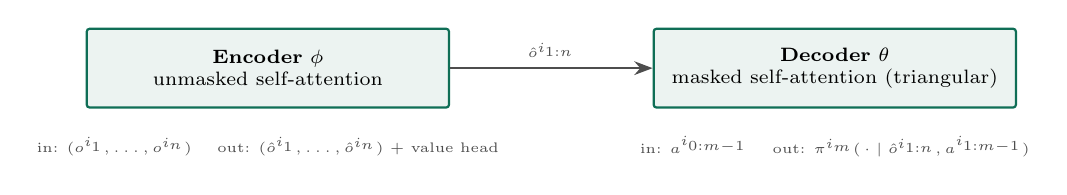
\begin{tikzpicture}[font=\scriptsize]
\node[draw=mDarkTeal, thick, fill=mDarkTeal!8, rounded corners=1pt, minimum width=4.6cm, minimum height=1.0cm, align=center] (enc) at (0,0) {\textbf{Encoder} $\phi$\\ unmasked self-attention};
\node[draw=mDarkTeal, thick, fill=mDarkTeal!8, rounded corners=1pt, minimum width=4.6cm, minimum height=1.0cm, align=center] (dec) at (7.2,0) {\textbf{Decoder} $\theta$\\ \alert{masked} self-attention (triangular)};
\node[mLightBrown, font=\tiny, align=center] at (0,-1.0) {in: $(o^{i_1},\dots,o^{i_n})$ \quad out: $(\hat o^{i_1},\dots,\hat o^{i_n})$ + value head};
\node[mLightBrown, font=\tiny, align=center] at (7.2,-1.0) {in: $a^{i_{0:m-1}}$ \quad out: $\pi^{i_m}(\,\cdot \mid \hat o^{i_{1:n}}, a^{i_{1:m-1}})$};
\draw[-{Stealth}, mLightBrown, thick] (enc) -- (dec) node[midway, above, font=\tiny]{$\hat o^{i_{1:n}}$};
\end{tikzpicture}
\end{center}
\smallskip
Two losses, trained jointly:
{\small
\begin{align*}
L_{\text{Enc}}(\phi) &= \tfrac{1}{Tn}\textstyle\sum_{m,t}\big[ R_t + \gamma V_{\bar\phi}(\hat o^{i_m}_{t+1}) - V_{\phi}(\hat o^{i_m}_{t}) \big]^2, \\[-2pt]
L_{\text{Dec}}(\theta) &= -\tfrac{1}{Tn}\textstyle\sum_{m,t} \min\big( r^{i_m}_t \hat A_t,\; \mathrm{clip}(r^{i_m}_t, 1\pm\epsilon)\, \hat A_t \big).
\end{align*}}
\smallskip
{\footnotesize The mask is the lemma in silicon: agent $i_m$ may attend to $a^{i_{1:m-1}}$, never to its successors.}
\end{frame}

\begin{frame}{MAT vs.\ HAPPO --- where the predecessors live}
\begin{center}\footnotesize\renewcommand{\arraystretch}{1.5}
\begin{tabular}{l|l|l}
 & \textbf{HAPPO} & \textbf{MAT} \\
\hline
predecessors enter via & correction factor $M^{i_{1:m}}$ (new ratios) & \alert{conditioning input} $a^{i_{1:m-1}}$ \\
advantage used & corrected $M$ & plain joint $\hat A_t$ \\
training & serial sweep (must wait) & \alert{parallel} (actions already in buffer) \\
inference & \alert{decentralized}, no comm ($o^i$ only) & centralized: others' \alert{realized} $a^{i_{1:m-1}}$ $+$ global obs \\
guarantee & monotonic improvement (Thm.\ 2) & same, via the decomposition (Thm.\ 1) \\
\end{tabular}
\end{center}
\medskip

\pause
\begin{block}{Remark --- this is \emph{centralized} execution, not decentralized}
Generating $a^{i_m}$ needs the predecessors' \alert{realized} actions $a^{i_{1:m-1}}$ \emph{and} the encoder's joint observations --- so MAT execution is \alert{centralized / communication-based}, \textbf{not} the no-communication decentralized execution of MAPPO/HAPPO. The price of parallel-trainable sequential decisions is execution-time communication: the \emph{learning-to-act} axis touches \emph{learning-to-communicate}.
\end{block}
\end{frame}

\begin{frame}{MAT --- evidence and positioning}
\begin{itemize}\setlength\itemsep{3pt}
\item \textbf{SMAC} (homogeneous teams): MAPPO is already strong, $\ge$ HAPPO.
\item \textbf{MAMuJoCo} (heterogeneous joints): HAPPO $>$ MAPPO --- heterogeneity rewards sequential, per-agent updates.
\item \textbf{MAT}: ahead in \alert{both} regimes; encoder--decoder beats encoder-only / decoder-only / GRU ablations; one-hot agent id beats positional encoding.
\end{itemize}
\medskip

\pause
Reading the pattern: parameter-shared simultaneous updates (MAPPO) suit \emph{interchangeable} agents; ordered updates (HAPPO/MAT) pay off precisely when agents are \emph{different} --- when the conflict that broke simultaneity is real.
\medskip
\pause
We now have three guaranteed algorithms. Are they three accidents --- or three points of one space?
\end{frame}

\begin{frame}{HAML --- zoom out: a template, three knobs}
\textbf{The answer: one template.} Those methods are not separate tricks. \textbf{Heterogeneous-Agent Mirror Learning} \paper{Zhong et al., JMLR 2024} shows every guaranteed algorithm so far --- HATRPO, HAPPO, MAT --- is one \emph{instantiation} of a single template, so the \alert{guarantee belongs to the template, not the trick}. An algorithm is then just a choice of \alert{three knobs}:
\medskip
\begin{itemize}\setlength\itemsep{3pt}
\item \textbf{drift functional} $\mathcal{D}^i$ --- a \emph{soft penalty} on moving away from the current policy (zero at no-move, zero gradient there);
\item \textbf{neighborhood operator} $\mathcal{U}^i$ --- a \emph{hard constraint} region around the current policy;
\item \textbf{sampling distribution} $\beta_{\pi}$ --- which states the update is averaged over.
\end{itemize}
\medskip
Update rule: agents in random order, each maximizing its drift-penalized expected advantage inside its neighborhood, conditioned on predecessors' new policies.
\medskip
\pause
{\footnotesize\textcolor{mLightBrown}{Next slide: the knob settings that recover HATRPO, HAPPO, \dots\ --- and the \emph{single} theorem that guarantees them all. (Formal operator HAMO: in the paper.)}}
\end{frame}

\begin{frame}{HAML --- instances, and the fundamental theorem}
\begin{center}\footnotesize\renewcommand{\arraystretch}{1.45}
\begin{tabular}{l|l|l|l}
\textbf{algorithm} & \textbf{drift} $\mathcal{D}^i$ & \textbf{neighborhood} $\mathcal{U}^i$ & \textbf{sampling} $\beta_\pi$ \\
\hline
HATRPO & $0$ & KL-ball ($\le\delta$) & on-policy \\
HAPPO & clip-based penalty & whole space & on-policy \\
HAA2C & $0$ & whole space & on-policy \\
HADDPG & $0$ & whole (deterministic) space & \alert{off-policy} (replay) \\
HATD3 & as HADDPG + TD3 tricks & --- & off-policy \\
\end{tabular}
\end{center}
\smallskip
\begin{block}{The Fundamental Theorem of HAML \hfill {\scriptsize\normalfont\paper{Zhong et al., 2024, Thm.\ 14}}}
\emph{Any} algorithm derived from the template enjoys, automatically:
(1) monotonic improvement of $J$; \; (2) $V_{\pi_k} \to V^{NE}$; \; (3) $J(\pi_k) \to J^{NE}$; \; (4) all $\omega$-limit points are Nash equilibria.
\end{block}
\end{frame}

\begin{frame}{The design pattern --- two menus, one course}
\begin{center}\footnotesize\renewcommand{\arraystretch}{1.5}
\begin{tabular}{l|l}
\textbf{Lecture 12's menu} & \textbf{Lecture 13's template} \\
\hline
choose: information structure $\times$ equilibrium concept & choose: drift $\times$ neighborhood $\times$ sampling \\
get: the right \emph{solution method} & get: an algorithm that \alert{inherits the guarantees} \\
guarantees: existence/uniqueness \emph{not} included & guarantees: monotonicity + NE convergence \emph{included} \\
\end{tabular}
\end{center}
\medskip

\pause
That is the quiet triumph of Stage 3: algorithm design became \textbf{menu selection in a space where every item is certified}.
\medskip

\pause
One question left on the strip --- and it is a question Lecture 12 never thought to ask, because back then reaching \emph{any} equilibrium was the dream:
\smallskip
\qstrip{5}
\end{frame}

%==========================================================
\section{Stage 4 --- which equilibrium? (2024)}
%==========================================================

\begin{frame}{Three residual problems of the standard objective}
NE convergence is not the end of the story. The \emph{standard} objective $\mathbb{E}[\sum\gamma^t r]$ has three residues:
\begin{itemize}\setlength\itemsep{3pt}
\item \textbf{exploration starves:} a deterministic optimal joint policy always exists, so stochasticity is never \emph{intrinsically} rewarded --- policies collapse early;
\item \textbf{lock-in:} with \alert{multiple} NEs, monotone improvement happily parks at a suboptimal one --- unilateral deviations are suppressed by design;
\item \textbf{cost:} on-policy sweeps (HAPPO) are sample-hungry; naive off-policy is unstable.
\end{itemize}
\medskip
\pause
The single-agent cure was \textbf{maximum entropy} RL (SAC). The multi-agent imports existed (FOP) --- but under an \alert{IGO assumption}.
\medskip
\pause
{\footnotesize\textcolor{mLightBrown}{Another assumption? We just spent a whole stage escaping one. Can MaxEnt come assumption-free?}}
\end{frame}

\begin{frame}{Recall --- single-agent maximum-entropy RL (SAC)}
\small
\textbf{The idea.} Maximize return \emph{plus} policy entropy --- reward for succeeding \emph{and} for staying as random as possible:
\[
J(\pi) = \mathbb{E}\Big[ \textstyle\sum_t r(s_t,a_t) + \alpha\,\mathcal{H}\big(\pi(\cdot\mid s_t)\big) \Big], \qquad \mathcal{H}(\pi)= -\mathbb{E}_{a\sim\pi}\log\pi(a\mid s).
\]
\textbf{Why.} The entropy bonus keeps \emph{exploration} alive, rewards \emph{robust} multi-modal behaviour, and stops early collapse to a brittle deterministic policy.
\medskip

\pause
\textbf{What changes.} The Bellman ``$\max$'' \emph{softens} into a log-sum-exp, and the optimal policy is no longer a hard $\arg\max$ but a \alert{Boltzmann} over $Q$:
\[
\pi^*(a\mid s) \;\propto\; \exp\!\big( Q_{\text{soft}}(s,a)/\alpha \big), \qquad V_{\text{soft}}(s) = \alpha \log\!\textstyle\sum_a e^{\,Q_{\text{soft}}(s,a)/\alpha}.
\]
\textbf{Temperature $\alpha$:} $\alpha\!\to\!0$ = ordinary greedy optimum (hard max); larger $\alpha$ = more random. \textbf{SAC} is the off-policy actor--critic that learns $Q_{\text{soft}}$ and pulls $\pi$ toward this Boltzmann target ($\alpha$ auto-tuned).
\medskip
\pause
{\footnotesize\textcolor{mLightBrown}{Lift this to $n$ agents next --- and the ``softened \emph{optimum}'' becomes a ``softened \emph{equilibrium}'' (QRE).}}
\end{frame}

\begin{frame}{The MaxEnt MARL objective}
\textbf{HASAC} \paper{Liu et al., ICLR 2024 Spotlight} \; augments the return with every agent's policy entropy:
\[
J(\bm\pi) \;=\; \mathbb{E}\Big[ \sum_{t} \Big( r(s_t,\mathbf{a}_t) \;+\; \alpha \sum_{i=1}^{n} \mathcal{H}\big(\pi^i(\cdot\mid s_t)\big) \Big) \Big].
\]
$\alpha$ is the \textbf{temperature}; \; $\alpha \to 0$ recovers the standard objective.
\medskip

\pause
\textbf{Where it comes from} {\footnotesize\textcolor{mLightBrown}{(origin annotation --- derivation not re-done here)}}: embed cooperative MARL in a probabilistic graphical model with optimality variables $p(O_t = 1 \mid s_t,\mathbf{a}_t) \propto e^{\,r(s_t,\mathbf{a}_t)}$; structured variational inference --- with the \emph{dynamics held fixed}, which is what prevents risk-seeking --- yields exactly this objective.
\medskip
\pause
Stochasticity is now part of \emph{what optimal means}. So: what is an ``equilibrium'' of this objective?
\end{frame}

\begin{frame}{QRE --- the equilibrium, softened}
\begin{block}{Theorem \hfill {\scriptsize\normalfont\paper{Liu et al., 2024, Thm.\ 1}}}
\centering
The equilibria of the MaxEnt objective are \textbf{quantal response equilibria}: each agent plays Boltzmann over its expected soft value,
\[
\pi^{i}_{\mathrm{QRE}}\big(a^i \mid s\big) \;\propto\; \exp\!\Big( \alpha^{-1}\, \mathbb{E}_{a^{-i}\sim \bm\pi^{-i}_{\mathrm{QRE}}}\big[ Q_{\bm\pi_{\mathrm{QRE}}}(s, a^i, a^{-i}) \big] \Big).
\]
\end{block}
\medskip

\begin{itemize}\setlength\itemsep{2pt}
\item QRE is the \alert{stochastic generalization of Nash} --- best responses smoothed by temperature. {\footnotesize\textcolor{mLightBrown}{(Game-theory callback: the logit / bounded-rationality equilibrium from our early lectures --- here it re-enters not as a model of human error, but as a \emph{design target}.)}}
\item $\alpha$ is a \textbf{dial}: $\alpha\!\to\!0$ recovers NE; larger $\alpha$ keeps exploration alive and resists premature lock-in.
\end{itemize}
\end{frame}

\begin{frame}{HASPI --- soft policy iteration, swept sequentially}
Two alternating steps --- the soft mirror of policy iteration:
\medskip

\textbf{(i) Joint soft policy evaluation.} Iterate the soft Bellman operator (a contraction):
\[
\Gamma_{\bm\pi} Q(s,\mathbf{a}) = r(s,\mathbf{a}) + \gamma\,\mathbb{E}_{s'}\big[ V(s') \big],
\qquad
V(s) = \mathbb{E}_{\mathbf{a}\sim\bm\pi}\Big[ Q(s,\mathbf{a}) + \alpha\textstyle\sum_i \mathcal{H}\big(\pi^i(\cdot\mid s)\big) \Big].
\]
\pause
\textbf{(ii) Sequential soft improvement.} In a random order, each agent KL-projects onto the Boltzmann of its \emph{conditional} soft value --- conditioned on predecessors' \alert{new} policies (the HAPPO sweep, soft edition).
\medskip
\pause
\begin{block}{Joint soft policy decomposition \hfill {\scriptsize\normalfont\paper{Liu et al., 2024, Prop.\ 1}}}
\centering
Composing the $n$ sequential local KL projections $=$ \emph{one} joint KL projection onto $\exp(Q/\alpha)/Z$:
\quad \alert{one MaxEnt MARL problem $=$ $n$ MaxEnt RL problems.}
\end{block}
\end{frame}

\begin{frame}{HASAC --- the algorithm, and what it promises}
\textbf{Practical recipe:} centralized soft critic $Q_\theta$ (Bellman residual); sequential per-agent policy updates by expected-KL minimization; reparametrization trick (continuous) / Gumbel--Softmax (discrete).
\medskip

\begin{itemize}\setlength\itemsep{2pt}
\item \textbf{Guarantees:} monotonic improvement of the MaxEnt objective, and convergence to \alert{QRE} --- with \textbf{no} IGO/IGM-style assumption.
\item \textbf{Generalization:} \emph{MEHAML} --- the MaxEnt mirror-learning template; \alert{HAML is exactly its $\alpha=0$ special case}. The whole Stage-3 edifice is one temperature away.
\item \textbf{Evidence:} best on \emph{31 of 35} tasks across six benchmarks, against HAPPO/HATRPO/MAPPO/QMIX/FOP/HATD3.
\end{itemize}
\medskip
\pause
{\footnotesize\textcolor{mLightBrown}{So HASAC \emph{is} HAML's machine: the \alert{sequential, predecessor-conditioned sweep is unchanged}. What changes is the \emph{destination} (Nash $\to$ QRE) and that sampling may be \emph{off-policy} (replay). The objective gained a term and the destination changed name --- the sweep did not.}}
\end{frame}

\begin{frame}{Stage 4 closed --- the concept became a dial}
Trace what ``equilibrium'' has been, across the course:
\begin{itemize}\setlength\itemsep{3pt}
\item \textbf{Lectures 1--7:} a \emph{definition} --- something you verify a strategy profile against.
\item \textbf{Lecture 12:} a \emph{menu column} --- a modeling choice that selects your solution method.
\item \textbf{Lecture 13, Stage 3:} a \emph{destination} --- something an algorithm provably converges to.
\item \textbf{Lecture 13, Stage 4:} a \alert{design dial} --- turn $\alpha$, and the destination itself moves smoothly from QRE toward NE.
\end{itemize}
\medskip
\pause
\begin{center}\large
The choice of concept never left the modeler's hands --- what changed is \alert{what the choice delivers}: from a definition to \emph{verify}, to a destination \emph{reached}, with a certificate.
\end{center}
\end{frame}

%==========================================================
\section{Finale --- the principle returns, and the course closes}
%==========================================================

\begin{frame}{Recall --- a dashed box we left in Lecture 8}
Lecture 8 ended its factorization arc with a \textbf{dashed} bridge: \emph{``DoF --- belongs to the policy-based story; we will pay this debt in Lecture 13.''}
\medskip

What stood on the solid side of that dash:
\[
\text{IGM:}\qquad \arg\max_{\mathbf{u}} Q_{tot} \;=\; \big( \arg\max_{u_1} Q_1,\, \dots,\, \arg\max_{u_N} Q_N \big)
\]
--- agreement of \emph{argmaxes}, bought with monotone mixing, so that a centralized value could be \textbf{executed decentralized}.
\medskip

\pause
Today's last stop asks IGM's question one more time --- in a setting Lecture 8 could not have imagined: \alert{when the policy itself is a generative model}.
\end{frame}

\begin{frame}{The fourth axis --- expressiveness}
Three axes carried this course. Today's papers quietly traced a \alert{fourth} --- the \textbf{function class} of actor and critic itself:
\smallskip
\begin{center}\scriptsize\renewcommand{\arraystretch}{1.4}
\begin{tabular}{l|l|l}
\textbf{function class} & \textbf{structural fact of the game it encodes} & \textbf{where we met it} \\
\hline
MLP & none --- a flat map & MADDPG's nets \\
RNN / GRU & \alert{partial observability}: compress the history $\tau$ & COMA's actor \\
GNN & permutation symmetry, sparse graph, variable $N$ & PIC (critic); MAMuJoCo / NerveNet kin \\
attention / Transformer & \alert{learned, dynamic} interaction weights & MAAC; MAT (agents as tokens) \\
diffusion & \alert{multimodal joint distributions}; action as a \emph{sample} & DoF (next) \\
\end{tabular}
\end{center}
\smallskip

\pause
\begin{itemize}\setlength\itemsep{1pt}
\item each step is an \textbf{inductive bias} answering one structural property of the game --- not fashion;
\item the axis is \alert{orthogonal to guarantees}: the mainline was sorted by \emph{what the update promises}, not by what the network is --- newer architecture $\neq$ better algorithm.
\end{itemize}
\smallskip
\pause
{\footnotesize The newest point on this line is generative --- where it lives, and what it breaks, next.}
\end{frame}

\begin{frame}{The new setting --- offline MARL, generative policies}
Two shifts since 2022:
\begin{itemize}\setlength\itemsep{3pt}
\item \textbf{Offline:} learn from a \emph{static log} of past behavior --- no exploration, no fresh rollouts. (The setting of real operations: plants, fleets, markets.)
\item \textbf{Generative policies:} \emph{diffusion models} represent rich, multimodal joint behavior far beyond a Gaussian head.
\end{itemize}
\medskip

\pause
\textbf{The CTDE problem returns, in generative costume.} A \emph{centralized} diffusion model over the joint action is expressive --- but it cannot be executed by separate agents. We need to \alert{factorize a generative model} the way we once factorized a value.
\medskip
\pause
And the factorization needs a principle --- an heir to IGM.
\end{frame}

\begin{frame}{DoF --- the IGD principle}
\textbf{DoF: a Diffusion Factorization framework for offline MARL} \paper{Li et al., ICLR 2025}
\medskip
\begin{block}{IGD --- Individual-Global-identically-Distributed}
\centering
The outcome \emph{generated} by the centralized diffusion model must be \textbf{identically distributed} to the \emph{collective} outcomes of the individual per-agent diffusion models.
\end{block}
\medskip

IGM matched \emph{argmaxes}; IGD matches \alert{distributions} --- the natural generalization when ``the policy'' is a sampler, not a maximizer.
\medskip

\pause
\textbf{Mechanism, at altitude:}
\begin{itemize}\setlength\itemsep{2pt}
\item \emph{noise factorization} --- split the centralized model's denoising noise across agents; provably satisfies IGD;
\item \emph{data factorization} --- model the residual inter-agent correlations the noise split leaves behind.
\end{itemize}
\end{frame}

\begin{frame}{One principle, three costumes}
\begin{center}
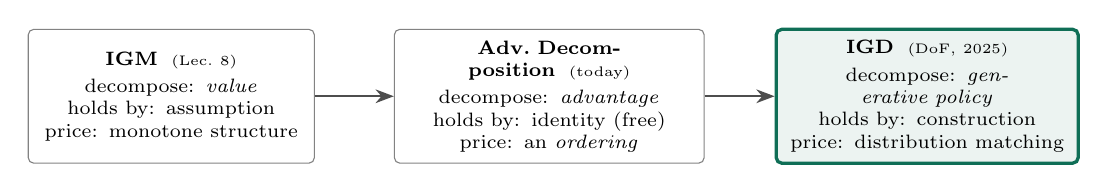
\begin{tikzpicture}[font=\scriptsize]
\node[draw=mLightBrown!70, rounded corners=2pt, align=center, text width=3.4cm, minimum height=1.7cm] (igm) at (0,0)
{\textbf{IGM} \;{\tiny(Lec.\ 8)}\\[2pt] decompose: \emph{value}\\ holds by: \alert{assumption}\\ price: monotone structure};
\node[draw=mLightBrown!70, rounded corners=2pt, align=center, text width=3.7cm, minimum height=1.7cm] (adv) at (4.8,0)
{\textbf{Adv.\ Decomposition} \;{\tiny(today)}\\[2pt] decompose: \emph{advantage}\\ holds by: \alert{identity} (free)\\ price: an \emph{ordering}};
\node[draw=mDarkTeal, very thick, fill=mDarkTeal!8, rounded corners=2pt, align=center, text width=3.6cm, minimum height=1.7cm] (igd) at (9.6,0)
{\textbf{IGD} \;{\tiny(DoF, 2025)}\\[2pt] decompose: \emph{generative policy}\\ holds by: \alert{construction}\\ price: distribution matching};
\draw[-{Stealth}, mLightBrown, thick] (igm) -- (adv);
\draw[-{Stealth}, mLightBrown, thick] (adv) -- (igd);
\end{tikzpicture}
\end{center}
\medskip

\pause
One question asked three times --- \emph{how can the joint thing be assembled from individual things?} --- and each era answered with the object it cared about: the value, the update, the sampler.
\medskip
\begin{center}
\alert{What we factorize evolved. The currency of the price changed. The question never did.}
\end{center}
\end{frame}

\begin{frame}{Diffusion --- policy, or planner?}
Diffusion enters MARL through \alert{two doors} --- and the course has seen this pair of doors before:
\smallskip
\begin{center}\footnotesize\renewcommand{\arraystretch}{1.35}
\begin{tabular}{l|l|l}
 & \textbf{diffusion policy} & \textbf{diffusion planner} \\
\hline
generates & an action, given the state & a whole joint \emph{trajectory} \\
executed as & a sampled rule $o \to a$ & plan $\to$ track $\to$ \alert{re-plan} (receding horizon) \\
lineage (Lec.\ 10/10) & \alert{feedback} / Eulerian & \alert{open-loop} / Lagrangian (Pontryagin) \\
exemplars & Diffusion-QL (2023); \alert{DoF} & Diffuser (2022); \alert{MADiff} (2024, attention across agents) \\
\end{tabular}
\end{center}
\smallskip

\pause
Lectures 9 and 10 return in generative clothing: the planner is a \emph{data-driven extremal generator}; as the re-planning horizon shrinks, it slides toward feedback --- the time-consistency dial, now a \alert{sampling schedule}.
\smallskip

\pause
\begin{block}{The open seam}
Ratio-based guarantees (HAPPO, HAML, HASAC) presume tractable $\log\pi$; diffusion policies sample easily but \alert{expose no likelihood}. At the frontier of expressiveness, the convergence certificates \textbf{re-open}. {\footnotesize(Hold this tension --- the next outlook ends the same way.)}
\end{block}
\end{frame}

\begin{frame}{The other axis --- act vs.\ communicate, formally}
We promised this at the spectrum slide. The two axes are two \emph{control architectures}, learned:
\smallskip
\begin{center}\footnotesize\renewcommand{\arraystretch}{1.5}
\begin{tabular}{l|l|l}
 & \textbf{learning to act} \;(today) & \textbf{learning to communicate} \\
\hline
execution information & $\eta^i = \{o_i\}$ & $\eta^i = \{o_i,\, m_{\mathcal{N}(i)}\}$ \\
control-theoretic kin & \alert{decentralized control} & \alert{distributed control} \\
computational shape & reactive pattern $o_i \to a_i$ & iterative \emph{consensus-like} inner loop \\
coordination paid & at training time (CTDE) & at execution time (messages) \\
objective structure & team, mixed, or competitive & (almost always) one team objective \\
\end{tabular}
\end{center}
\smallskip

\pause
The consensus reading is literal, not poetic: CommNet's channel is
\[
c_j \;=\; \tfrac{1}{J-1}\textstyle\sum_{j'\neq j} h_{j'} \quad\text{--- the \alert{average-consensus operator}, iterated $K$ times before acting.}
\]
\smallskip
{\footnotesize\textcolor{mLightBrown}{Terminology varies across communities (in ML, ``distributed'' often just means parallel hardware); we have used the control-theoretic sense.}}
\end{frame}

\begin{frame}{The other axis --- a one-slide genealogy, and a thesis}
The communicate axis has its own question chain --- a future lecture of its own:
\medskip
\begin{center}\footnotesize
\emph{can a channel be learned?} $\to$ CommNet (2016) $\to$ BiCNet (2017) $\to$
\emph{when to speak?} $\to$ ATOC (2018), IC3Net (2019) $\to$
\emph{to whom?} $\to$ TarMAC (2019) $\to$
\emph{under bandwidth/contention constraints?} $\to$ SchedNet (2019)
\end{center}
\medskip

\pause
\begin{block}{Thesis for that lecture}
\centering
\textbf{Learned distributed control:} learn the \emph{protocol} itself --- and pay for it with the loss of classical consensus \emph{guarantees}.
\end{block}
\medskip
\pause
{\footnotesize And remember where today's axis already touched it: MAT's autoregressive action-passing \emph{is} one round of communication. The two axes are a spectrum, not a wall.}
\smallskip

{\footnotesize \alert{Two outlooks, one shape:} expressiveness re-opens \emph{convergence} guarantees; communication surrenders \emph{consensus} guarantees. Both futures begin exactly where today's certificates end.}
\end{frame}

\begin{frame}{The course map, complete}
\begin{center}\footnotesize
\renewcommand{\arraystretch}{1.7}
\begin{tabular}{r|c|c}
 & \textbf{Single Agent} & \textbf{Multi Agent} \\
\hline
\textbf{Static}  & Static optimization \;{\scriptsize\checkmark} & Static games \;{\scriptsize Lec.\ 1--5 \checkmark} \\
\hline
\textbf{Dynamic, discrete} & MDP / value RL \;{\scriptsize Lec.\ 6 \checkmark} & Stochastic games / value MARL \;{\scriptsize Lec.\ 7--8 \checkmark} \\
\hline
\textbf{Dynamic, continuous} & Optimal control / policy RL \;{\scriptsize Lec.\ 10 \checkmark} & \cellcolor{mDarkTeal!15} Diff.\ games / \textbf{policy MARL} \;{\scriptsize Lec.\ 12--11 \checkmark}\\
\end{tabular}
\end{center}
\medskip

\pause
And across every cell, one repeated journey: \;\textbf{model} $\to$ \textbf{data}; \;\textbf{minimize} $\to$ \textbf{standoff}; \;\textbf{assume} $\to$ \alert{\textbf{prove}}.
\end{frame}

\begin{frame}{Closing --- the one sentence}
\vfill
\begin{center}\large
Lecture 12 wrote the equations of the standoff.\\[8pt]
Lecture 13 learned to \alert{reach} it ---\\[4pt]
without the model, \;with a proof,\\[4pt]
and finally, with a \alert{choice of which standoff to reach}.
\end{center}
\vfill
\pause
\footnotesize
From $(0.5)^N$ gradients to QRE convergence in seven years: the distance between \emph{hoping} the agents coordinate and \emph{certifying} that they will. That certificate is what this course was for.
\end{frame}

\begin{frame}[standout]
Questions?
\end{frame}

%==========================================================
\appendix
%==========================================================

\begin{frame}{Backup 1 --- why $(0.5)^N$: the signal-starvation sketch}
\footnotesize
\textbf{Setting} \paper{Lowe et al., 2017, Prop.\ 1}: $N$ agents, $a_i \in \{0,1\}$ with $P(a_i{=}1)=\theta_i$; reward $r = \mathbf{1}\{a_1 = \cdots = a_N = 1\}$; uninformed initialization $\theta_i = 0.5$ (the worst-case construction stated in the main deck).
\medskip

\textbf{Step 1 --- when is a sample informative?} The REINFORCE estimate $\hat\nabla J = \nabla\log\pi(\mathbf{u})\, r(\mathbf{u})$ is nonzero only when $r\neq 0$ --- i.e.\ when all $N$ agents \emph{simultaneously} act correctly. Under uniform play: probability $(0.5)^N$.
\medskip

\textbf{Step 2 --- what do the other samples do?} They contribute exactly $0$ to the estimate --- no correction, just dilution: the estimator is a sea of zeros with rare informative spikes.
\medskip

\textbf{Step 3 --- direction.} With single (or few) samples, $\langle\hat\nabla J, \nabla J\rangle > 0$ requires catching a spike; hence
\[
P\big(\langle\hat\nabla J,\nabla J\rangle > 0\big) \;\propto\; (0.5)^N .
\]
\medskip
\textbf{Moral:} the problem is not variance around the right direction --- it is that \alert{informative coordination events vanish exponentially}. A centralized critic, conditioning on all actions, restores per-sample signal.
\end{frame}

\begin{frame}{Backup 2 --- the counterfactual baseline adds zero bias, in full}
\footnotesize
Claim: $\displaystyle \mathbb{E}_{\mathbf{u}\sim\bm\pi}\Big[ \nabla_\theta \log \pi^i(u^i\mid\tau^i)\; b\big(s,\mathbf{u}^{-i}\big) \Big] = 0$ \, where $b(s,\mathbf{u}^{-i}) = \sum_{u'^i}\pi^i(u'^i|\tau^i)\, Q(s,\boldsymbol\tau,(\mathbf{u}^{-i},u'^i))$.
\medskip

\textbf{Step 1 --- factor the joint expectation.} $\bm\pi(\mathbf{u}) = \pi^{-i}(\mathbf{u}^{-i})\,\pi^i(u^i|\tau^i)$, and $b$ does not contain $u^i$:
\[
\mathbb{E}_{\mathbf{u}}[\,\cdot\,] = \sum_{\mathbf{u}^{-i}} \pi^{-i}(\mathbf{u}^{-i})\; b(s,\mathbf{u}^{-i}) \underbrace{\sum_{u^i} \pi^i(u^i|\tau^i)\, \nabla_\theta\log\pi^i(u^i|\tau^i)}_{\text{inner sum}}.
\]
\textbf{Step 2 --- likelihood-ratio identity} ($\pi\nabla\log\pi = \nabla\pi$): inner sum $= \sum_{u^i} \nabla_\theta\, \pi^i(u^i|\tau^i)$.
\medskip

\textbf{Step 3 --- exchange sum and gradient, use normalization:} $\sum_{u^i}\nabla_\theta\pi^i = \nabla_\theta \sum_{u^i}\pi^i = \nabla_\theta\,1 = 0$. Hence the whole expression is $0$. \hfill$\blacksquare$
\medskip

\textbf{Remark.} The proof used only one property of $b$: \alert{independence from the sampled $u^i$}. Freezing $\mathbf{u}^{-i}$ keeps that property while making $b$ maximally informative about teammates --- the best of both.
\end{frame}

\begin{frame}{Backup 3 --- the telescoping proof, fully expanded}
\footnotesize
Definitions (convention $Q^{i_{1:0}}_\pi := V_\pi(s)$):
\[
Q^{i_{1:m}}_{\pi}(s,\mathbf{a}^{i_{1:m}}) = \mathbb{E}_{\mathbf{a}^{-i_{1:m}}\sim\pi}\big[Q_\pi(s,\mathbf{a})\big],
\qquad
A^{i_j}_{\pi}(s,\mathbf{a}^{i_{1:j-1}},a^{i_j}) = Q^{i_{1:j}}_{\pi}(s,\mathbf{a}^{i_{1:j}}) - Q^{i_{1:j-1}}_{\pi}(s,\mathbf{a}^{i_{1:j-1}}).
\]
Sum over $j = 1,\dots,n$ and write every term out:
\begin{align*}
\sum_{j=1}^{n} A^{i_j}_{\pi}
&= \big( Q^{i_{1:1}} - Q^{i_{1:0}} \big) + \big( Q^{i_{1:2}} - Q^{i_{1:1}} \big) + \big( Q^{i_{1:3}} - Q^{i_{1:2}} \big) + \cdots + \big( Q^{i_{1:n}} - Q^{i_{1:n-1}} \big) \\
&= Q^{i_{1:n}}_{\pi}(s,\mathbf{a}) - Q^{i_{1:0}}_{\pi}(s) \;=\; Q_{\pi}(s,\mathbf{a}) - V_{\pi}(s) \;=\; A^{i_{1:n}}_{\pi}(s,\mathbf{a}). \qquad\blacksquare
\end{align*}
\medskip
\textbf{Why no assumption is needed:} every $Q^{i_{1:m}}$ is \emph{defined} by marginalizing the same one joint $Q_\pi$ --- we never asked $Q_\pi$ to decompose; we only sliced its expectations along an ordering. The ordering is the entire ``cost.''
\medskip

\textbf{Same identity, observation-based} \paper{MAT, Thm.\ 1}: replace $s$ by joint observation $\mathbf{o}$ throughout; nothing changes.
\end{frame}

\begin{frame}{Backup 4 --- single-agent TRPO recap}
\small
\textbf{Lemma $\to$ surrogate.} The true gain $J(\pi_{\text{new}})-J(\pi_{\text{old}}) = \mathbb{E}_{s\sim\rho_{\text{new}},\,a\sim\pi_{\text{new}}}[A_{\pi_{\text{old}}}(s,a)]$ uses the \emph{new} state distribution $\rho_{\text{new}}$. For nearby policies $\rho_{\text{new}}\approx\rho_{\text{old}}$, giving an objective computable from the \emph{old} batch:
\[
L(\theta) = \mathbb{E}_{s\sim\rho_{\text{old}},\,a\sim\pi_{\text{old}}}\big[\, r(\theta)\, A(s,a)\,\big], \qquad r(\theta)=\frac{\pi_\theta(a\mid s)}{\pi_{\theta_k}(a\mid s)}.
\]
\textbf{Importance ratio $r$.} It reweights each old sample by how much more/less the \emph{new} policy would take that action ($r>1$: more likely). It is the \emph{only} $\theta$-dependent factor, so maximizing $\mathbb{E}[rA]$ simply raises the probability of high-advantage actions.
\smallskip

\textbf{Trust region.} $\mathbb{E}_s[D_{\mathrm{KL}}(\pi_{\theta_k},\pi_\theta)]\le\delta$ keeps the policies close $\Rightarrow$ the $\rho$-approximation holds, $r$ stays bounded (variance control), and improvement is \emph{monotonic} --- the surrogate lower-bounds the true gain.
\smallskip

\textbf{Closed form.} Linearize $L$ ($g=\nabla_\theta L$), quadratize the KL (Fisher $H$) $\Rightarrow$ natural-gradient step
\[
\theta_{k+1} = \theta_k + \sqrt{\tfrac{2\delta}{g^\top H^{-1} g}}\; H^{-1} g \qquad (+\ \text{backtracking line search}).
\]
{\footnotesize\textcolor{mLightBrown}{HATRPO is this \emph{verbatim}, with $A\to M^{i_{1:m}}$ (the predecessor-corrected joint advantage) and $r\to r^{i_m}$.}}
\end{frame}

\begin{frame}{Backup 5 --- HATRPO's closed-form step}
\footnotesize
Problem at agent $i_m$: \; $\max_{\theta}\, L(\theta) := \mathbb{E}[(r^{i_m}(\theta)-1)M^{i_{1:m}}]$ \; s.t.\ \; $\bar D_{KL}(\theta_k, \theta) \le \delta$.
\medskip

\textbf{Step 1 --- local models at $\theta_k$.} Linearize the objective and quadratize the constraint:
\[
L(\theta) \approx g^{\top}(\theta - \theta_k), \qquad
\bar D_{KL}(\theta_k,\theta) \approx \tfrac12 (\theta-\theta_k)^{\top} H\, (\theta-\theta_k),
\]
with $g = \nabla_\theta L|_{\theta_k}$ and $H$ the Hessian of the expected KL (the Fisher matrix).
\medskip

\textbf{Step 2 --- maximize a linear function on an ellipsoid.} The optimum lies on the boundary, along the natural-gradient direction $H^{-1}g$; scaling to KL-radius $\delta$ gives
\[
\theta_{k+1} = \theta_k + \sqrt{\tfrac{2\delta}{\,g^{\top}H^{-1}g\,}}\; H^{-1}g.
\]
\textbf{Step 3 --- practice.} $H^{-1}g$ by conjugate gradient (never form $H$); multiply by backtracking coefficient $\alpha^{j} < 1$ until the \emph{actual} (non-approximated) constraint and improvement hold.
\medskip

\textbf{What is multi-agent here?} Only $M^{i_{1:m}}$ --- the predecessors' importance correction inside $g$. The trust-region machinery itself is Lecture 10's, untouched.
\end{frame}

\begin{frame}{Backup 6 --- soft machinery notes (HASAC)}
\footnotesize
\textbf{Soft policy evaluation converges} \paper{Liu et al., 2024, Lem.\ 4.1}: with bounded rewards and bounded entropy (finite action spaces / regular policies), the soft Bellman operator
$\Gamma_{\bm\pi}Q = r + \gamma\,\mathbb{E}[V]$, $V = \mathbb{E}_{\bm\pi}[Q + \alpha\sum_i\mathcal{H}(\pi^i)]$
is a $\gamma$-contraction in the sup norm (the entropy enters as a bounded per-step bonus), so iterating it converges to the unique soft $Q_{\bm\pi}$.
\medskip

\textbf{QRE exists.} The QRE condition is a fixed point of the smooth map $\bm\pi \mapsto$ (per-agent Boltzmann responses); on the compact convex product of simplices, continuity gives existence (Brouwer). Smoothing is what buys this --- compare Lecture 12, where existence of (exact) equilibria was one of the three honest warnings.
\medskip

\textbf{The $\alpha \to 0$ limit.} As temperature vanishes, QREs concentrate on (a selection of) Nash equilibria --- the dial meets the Stage-3 destination. For fixed $\alpha > 0$, payoffs are entropy-perturbed: the equilibrium reached is \emph{intentionally} not the deterministic NE.
\medskip

\textbf{Template view} \paper{MEHAML, Thm.\ 3}: drift, neighborhood, and sampling knobs as in HAML; any derived algorithm gets monotonic improvement and QRE convergence; HAML $=$ MEHAML at $\alpha = 0$.
\end{frame}

\end{document}
